\documentclass[oneside]{ausarbeitung}
\bibliography{latexlit}

\usepackage{float}
\usepackage{url}
\usepackage{listings}
\usepackage{algorithm} 
\usepackage{algpseudocode}

% ----------------------------------------------------------------------

\begin{document}

%--- Sprachauswahl
% Erlaubte Werte:
%   \selectlanguage{english}
%   \selectlanguage{ngerman}
\selectlanguage{ngerman}

%--- Art der Arbeit
% Erlaubte Werte:
%   \Praxissemesterbericht
%   \Projektbericht
%   \Bachelorarbeit
%   \Seminararbeit
%   \Masterarbeit

\Projektbericht

%--- Studiengang:
% Erlaubte Werte:
%   \Informatik
%   \Elektronik
%   \DataScience
\Informatik

\title{Algorithmisches Handeln von Kryptowährungen}

\author{Sebastian Flum}
\matrikelnr{76855}

%--- Ist der Erstbetreuer (\examinerA) an der Hochschule ein Professor?
% Erlaubte Werte:
%   \examinerIsAProfessortrue   % Ja
%   \examinerIsAProfessorfalse  % Nein
\examinerIsAProfessorfalse

%--- Betreuer
\examinerA{Sebastian Stigler}
%\examinerB{Prof.~Dr.~Ulrich~Klauck}

%--- Einreichungsdatum
\date{28. Februar 2021}

%--- Titelseite Anzeigen
\maketitle
\cleardoublepage

%---
\pagenumbering{roman}
\setcounter{page}{1}

%--- Eidesstattliche Erklärung anzeigen
\makeaffirmation
\cleardoublepage

%---------------------------------------------------
\begin{abstract}
\label{abstract}

Beim algorithmischen Handeln werden Handelsentscheidungen auf der
Grundlage zuvor definierter Anweisungen und Regeln getroffen, die in
Form eines Computerprogramms umgesetzt wurden. Dabei wird Code
geschrieben, der die Trades im Namen des Händlers oder Investors
ausführt, wenn bestimmte Bedingungen erfüllt sind.  

Im Rahmen dieser Arbeit wurde versucht, jenes Verfahren auf den Handel
von kryptographischen Währungen wie Bitcoin oder Ethereum anzuwenden
und den Grundstein eines algorithmisches Handelssystem für diese zu
entwerfen. So soll herausgefunden werden, ob der automatisierte Handel
von Kryptowährungen, durch ein selbst entwickeltes System,
erfolgreich sein kann.

Dabei beschäftigt sich diese Arbeit im grundlegenden mit folgenden Konzepten:

\begin{enumerate}
	\item Algorithmische Handelsstrategien und technische Indikatoren
	\item Implementierung einer Schnittstelle für Handelsplattformen
	\item Backtesting von Handelsstrategien
	\item Entwurf und Verwaltung eines Trading Bots
	\item Erstellung einer Konsolenanwendung
	\item Verknüpfung dieser Elemente innerhalb eines modularen Systems
\end{enumerate}

Umgesetzt wurde dieses Projekt fast ausschließlich unter der
objektorientierten Verwendung der Programmiersprache Python, in
Verbindung mit einigen wenigen HTML Elementen.

\end{abstract}

%---------------------------------------------------
\cleardoublepage
\tableofcontents

%---
\listoffigures

%---
\listoftables

%---
\listoflistings

%---
\listofabbreviations
\begin{acronym}[API]  % Längstes Kürzel in der nachfolgenden
                       % Liste um die Breite der Spalte für die
                       % Abkürzungen zu bestimmen.

%% Eintrag: \acro{Referenzname}[Kürzel]{Langform}
%% Im Text wird die Abkürzung dann mit \ac{Referenzname} benutzt.
\acro{api}[API]{Application Programming Interface}
\acro{sma}[SMA]{Simple Moving Average}
\acro{cfd}[CFD]{Contract for Difference}
\acro{rest}[REST]{Representational State Transfer}
\acro{http}[HTTP]{Hypertext Transfer Protocol}
\acro{pandas}[Pandas]{Python Data Analysis Library}
\acro{url}[URL]{Uniform Resource Locator} 
\acro{json}[JSON]{JavaScript Object Notation}
\acro{abc}[ABC]{Abstract Base Class}
\end{acronym}
%---


\cleardoublepage
\pagenumbering{arabic}
\setcounter{page}{1}

%---------------------------------------------------
\chapter{Einleitung}
\label{cha:einleitung}

"Neues Allzeithoch: Bitcoin-Rekordjagd geht ungebremst
weiter"\cite{bitcoin_artikel_1}. "Kryptowährung: Bitcoin knackt Marke
von 50.000 Dollar"\cite{bitcoin_artikel_2}. Artikel wie diese sind
schon lange keine Seltenheit mehr. Kryptowährungen, allen voran der
Bitcoin, entwickelten sich in den letzten Jahren zum Sinnbild
schnellen Reichtums. Doch das war nicht immer so. Im Jahre 2011, als
sich der Bitcoin noch in seinen Kinderschuhen befand, kostete ein Coin
gerade einmal 1 Dollar\cite{bitcoin_kurs_2011}. Vielleicht erwischt
man sich nun selbst bei dem Gedanken daran, was wohl wäre, wenn man
zu dieser Zeit schon das Potential dieser, damals unscheinbaren,
Internetwährung erkannt hätte. Einige vorausdenkende Köpfe
erkannten dies frühzeitig und wurden dadurch reich. Andere wiederum
nutzten die neu entdeckte Kryptowährung dazu, online für ihre Pizza
zu bezahlen. Verrückt, wenn man sich vor Augen führt, dass man mit
der selben Menge Bitcoins heute zehntausende Pizzen bezahlen könnte.
Vielleicht lässt dieser Gedanke die Herzen einiger Pizzaliebhaber
höher schlagen, vorrangig stellt sich jedoch die Frage, ob man mit
dem Besitz und Handel von Kryptowährungen heutzutage noch Erfolg
haben kann. Und wenn ja - kann das auch ein Computerprogramm?


\section{Motivation}
\label{sec:motivation}

Natürlich stellt die Aussicht auf realisierbaren Gewinn, erzeugt
durch ein selbst entwickeltes Handelssystem, ein großer
Motivationsfaktor dar - doch es ist mehr als das. Kryptowährungen
liegen einem faszinierendem Stück Technologie zugrunde. Der
sogenannten \textbf{Blockchain} (dazu später mehr). Dennoch können
die digitalen Währungen wie jede herkömmliche Währung getauscht und
gehandelt werden, befinden sich gleichzeitig aber außerhalb der
Kontrolle finanzieller Institutionen. Somit verbinden Kryptowährungen
die Welt des Finanzhandels mit der Welt der Informatik. Für jemanden,
den der herkömmliche Handel mit Wertpapieren oder Ähnlichem nur
wenig anspricht, bieten Kryptowährungen die Möglichkeit eines
interessanten Einblicks in beide Welten. 

Abgesehen davon finde ich großen Gefallen daran, Lösungen für
gegebene Problemstellungen zu entwerfen und in Programmcode
umzusetzen. Es macht mir Spaß, neue Technologien kennenzulernen und
deren Konzepte praktisch einzusetzen. Der Entwurf eines
algorithmischen Handelssystems bietet dafür die perfekte Grundlage,
da es beliebig erweitert werden kann und viele Schlüsselkonzepte
vereint. So stellt das Projekt eine interessante Möglichkeit für
mich dar, Dinge wie objektorientierte Programmierung, Entwurf von
Softwarearchitekturen und Datenbanken, Web-Entwicklung und vielem
mehr, innerhalb eines zusammenhängenden Projektes, kennenzulernen und
anzuwenden.


\section{Problemstellung und -abgrenzung}
\label{sec:problemstellung}

Als Ganzes betrachtet ist die Problemstellung, ein algorithmisches
Handelssystem zu entwerfen, relativ unüberschaubar. Zur Bewältigung
muss es daher in mehrere Teilprobleme heruntergebrochen werden. Daraus
ergeben sich folgende, im nachfolgenden grob beschriebene,
Problemstellungen:

\textbf{1. Algorithmische Handelsstrategien und technische Indikatoren} \\
Ohne eine geeignete Trading Strategie, die entscheidet, wann Einkäufe
und Verkäufe zu tätigen sind, kann wohl kein System Erfolg haben.
Diesen Trading Strategien liegen technische Indikatoren zu Grunde. Ein
technischer Indikator dient dabei zur alternativen Darstellung der
Kursverläufe und liefert der Strategie wertvolle Analyseinformationen.
Der Fokus soll dabei jedoch weniger auf der Findung und Konzeption
neuer Strategien und Indikatoren liegen, sondern darauf, wie diese
möglichst einfach und modular in das System eingebunden werden
können.

\textbf{2. Entwurf einer Schnittstelle für Handelsplattformen} \\
Der Handel von Kryptowährungen mittels eines algorithmischen Systems
erfordert, genauso wie beim Handeln von Hand, eine Plattform, auf der
die Ein- und Verkäufe getätigt werden. Im Vergleich zum Handeln von
Hand, benötigt das Trading-System jedoch ein \ac{api}, an die es
anknüpfen kann, um mögliche Aktionen der Plattform tätigen zu
können. Einige Plattformen bieten solche APIs zum Teil kostenlos an.
Die Problemstellung ergibt sich daraus, die von den Plattformen
bereitgestellten APIs zu nutzen und eigene, möglichst modulare,
Schnittstellen zur Verwendung dieser zu entwerfen.

\textbf{3. Backtesting von Handelsstrategien} \\
Backtesting bzw. Rückvergleich bezeichnet den Prozess, eine Strategie
zu evaluieren, indem die Strategie auf historische Daten angewandt
wird\cite{backtesting_definition}. Findet man beispielsweise eine neue,
vielversprechende Trading
Strategie und möchte diese nun nach der Umsetzung in Code testen, ist
es sehr riskant, die Strategie im Echtzeitbetrieb laufen zu lassen.
Sollte die Strategie nämlich doch nicht so vielversprechend sein,
läuft man Gefahr, große Verluste durch schlecht platzierte Ein- und
Verkäufe hinnehmen zu müssen. Der Backtest wirkt diesem Risiko
entgegen und stellt somit eine der wichtigsten Komponenten des Systems
dar.

\textbf{4. Entwurf und Verwaltung eines Trading Bots} \\
Echzeitdaten auswerten und automatisiert Einkäufe und Verkäufe
tätigen zu lassen. Da dies den Umfang dieser Arbeit jedoch
übersteigt, soll innerhalb dieses Projekts nur der Grundstein dieses
Features gelegt werden.

\textbf{5. Erstellung einer Konsolenanwendung} \\
Alle Features des zu entwickelnden Systems, sollen dem Nutzer als Teil
einer Konsolenanwendung zur Verfügung stehen. Mit dieser soll es
beispielsweise möglich sein, Backtests sowie neue
"Händler-Instanzen" aka Trading-Bots zu erstellen, welche
verschiedenen Parametern wie Auswahl der Kryptowährung, Strategie,
Kapital, usw. zu Grunde liegen.

\textbf{6. Verknüpfung der Komponenten innerhalb eines modularen Systems} \\
Im laufe der Arbeit werden Lösungskonzepte für die, hier
aufgeführten, Problemstellungen entworfen und implementiert. Wichtig
ist es dabei, die Komponenten mit Hinblick auf das Gesamtsystem und
dessen Erweiterbarkeit/Modularität zu entwerfen, sowie ein sauberes
und klar definiertes Zusammenspiel zu ermöglichen. 

\section{Ziel der Arbeit}
\label{sec:ziel}

Wie sich aus den vorherigen Abschnitten bereits erkennen lässt,
stellt das Ziel dieser Arbeit den Entwurf und die Implementierung
eines algorithmischen Handelssystems für Kryptowährungen dar. Dabei
soll es dem System möglich sein, Marktdaten über Kryptowährungen zu
sammeln und automatisiert auszuwerten. Des weiteren soll das System
über eine Teststrategie sowie den dazugehörigen technischen
Indikatoren enthalten, welche durch einen, ebenfalls im System
implementierten, Backtest ausgewertet werden kann. Dabei soll es dem
System möglich sein, ausgewählte Markdaten und Backtest-Ergebnisse
zu visualisieren und anschaulich darzustellen. Unter anderem soll das
System einen Prototyp eines Trading-Bots enthalten, welcher mit
zukünftigen Erweiterungen in der Lage sein soll, echte
Handelsaktionen durchzuführen. Diese Handelsaktionen werden innerhalb
dieser Arbeit jedoch \underline{nicht} implementiert, d.h. das System
ist innerhalb diesen Projekts nicht in der Lage, eigenständig reale
Käufe und Verkäufe zu tätigten. Die zuvor genannten Funktionen
sollen dem Nutzer letztendlich durch eine Konsolenanwendung
bereitgestellt werden.

\section{Vorgehen}
\label{sec:vorgehen}

Nachdem mit Problemstellung und Ziel gewissermaßen Anfangs- und Endpunkt 
des Praktikums beschrieben sind, wird hier der zur Erreichung des Ziels 
eingeschlagene Weg vorgestellt. Dazu werden typischerweise die folgenden 
Kapitel und ihr Beitrag zur Erreichung des Ziels der Arbeit kurz 
beschrieben. Die folgenden Kapitel sind ein – möglicher – Aufbau, 
Abweichungen können durchaus notwendig sein. Zur Darstellung des 
Vorgehens ist eine grafische Darstellung sinnvoll, bei der die einzelnen 
Lösungsschritte und ihr Zusammenhang dargestellt werden. Ein Beispiel 
hierfür findet sich in Abbildung \ref{fig:1}.

\begin{figure}[htbp]
  \centering
  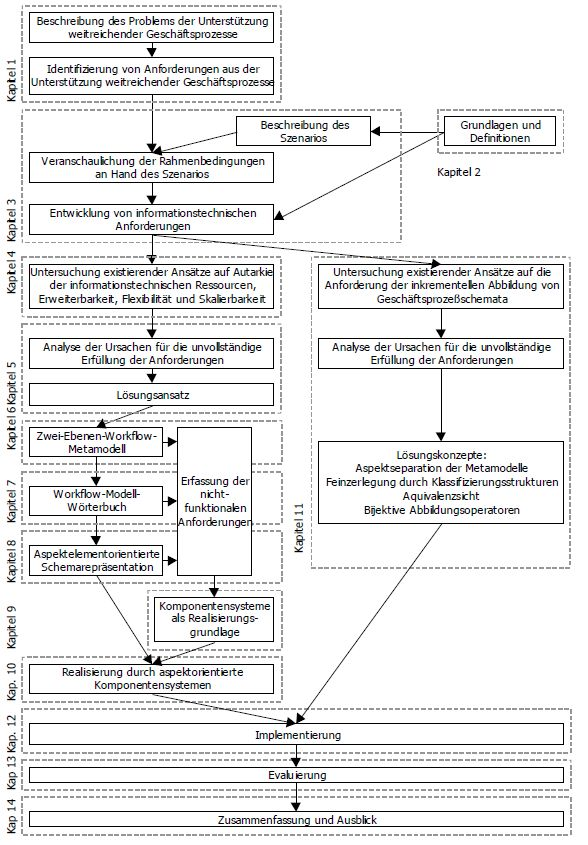
\includegraphics[height=0.9\textheight]{img/ausarbeitung.jpg}
  \caption{vorgehen nach \autocite{Schmidt:Geschaeftsprozesse}}
  \label{fig:1}
\end{figure}

%---------------------------------------------------
\chapter{Grundlagen}
\label{cha:grundlagen}

%----
\section{Trading}
\label{sec:trading}

Das Wort "Trading", zu Deutsch: Handel, stammt aus dem Englischen und
beschreibt den Kauf und Verkauf von Finanzprodukten an einer Börse.
Menschen, die dieser Beschäftigung nachgehen, werden daher auch als
Trader bezeichnet. Ein durchgeführter Handel heißt dementsprechend
also Trade. (vgl. \cite{trading_1})

Trading bedeutet, die Schwankungen der Finanzmärkte mithilfe von
Trades für die eigenen Zwecke zu nutzen. Das heißt kaufen, verkaufen
und dabei Gewinne einstreichen - oder den Verlust verkraften. Durch
das Internet und benutzerfreundliche Trading-Anbieter ist es auch für
Hobby-Anleger möglich, Finanzinstrumente wie Wertpapiere, Währungen,
Rohstoff-Zertifikate oder Ähnlichem zu handeln. Beim Trading handelt
es sich grundsätzlich um Spekulation. Wo ein Trader sein Geld
investiert, ist meist von untergeordneter Wichtigkeit. Beispielsweise
geht es nicht darum, Anteile eines Unternehmens zu kaufen, um
langfristig an dessen Entwicklung teilzuhaben. Das Ziel eines Traders
ist es, durch einen Kursanstieg im Zeitraum des Besitzes eins
Finanzinstruments Gewinn zu erzielen. Das bedeutet, ein Trader kauft
beispielsweise eine Aktie, hofft auf einen Kursanstieg und verkauft
sie dann wieder. Die anschließende Wertdifferenz abzüglich der
Transaktionskosten stellt den Gewinn des Traders dar. (vgl.
\cite{trading_2})

\subsection{Order Types}
\label{sub:Order Types}

Mit der verbreitung der digitalen Technologie und des Internets entscheiden sich viele Anleger dafür, Aktien selbst online zu kaufen und zu verkaufen, anstatt Beratern hohe Provisionen für die Ausführung von Geschäften zu zahlen. Beim Platzieren eines Auftrags bzw. Order stehen dem Trader mehrere verschiedene Order-Types zur Verfügung.

\textbf{Market Orders} \\
Eine Market Order ist die grundlegendste Art des Handels. Es ist ein Auftrag zum sofortigem Kauf oder Verkauf zum aktuellen Kurs. Kauft man eine Aktie, zahlt man in der Regel einen Preis zum oder in der Nähe des veröffentlichten Briefkurses. Wenn eine Aktie verkauf werden soll, erhält man einen Preis zum oder in der Nähe des eingestellten Geldkurses.

\textbf{Stop-Loss Order} \\
Eine Stop-Loss Order ist eine der nützlichsten davon. Diese Order unterscheidet sich von anderen Orders, denn im Gegensatz zu Markt Orders, die aktiv sind, sobald sie eingegeben werden, bleibt diese Order ruhend, bis ein bestimmter Preis überschritten wird. Erst dann wird sie als Market Order aktiviert.

Wenn zum Beispiel eine Stop-Loss Order auf die XYZ-Aktien bei 45€ pro Aktie platziert würde, wäre die Order inaktiv, bis der Preis 45€ erreicht oder unterschritten hat. Die Order würde dann in eine Market Order umgewandelt und die Aktien würden zum besten verfügbaren Preis verkauft werden. Man sollte diese Art von Order in Betracht ziehen, wenn man keine Zeit hat, den Markt ständig zu beobachten, aber Schutz vor einer großen Abwärtsbewegung benötigt. (vgl. \cite{order_types})

\subsection{Algorithmischer Handel}
\label{sub:algorithmischer_handel}

Algorithmischer beschreibt den automatischen Handel von
Finanzinstrumenten durch Computerprogramme. Dabei folgt das
Computerprogramm einem vordefiniertem Satz von Anweisungen
(Algorithmus), um einen Trade zu platzieren. Die Trades können
theoretisch Gewinne mit einer Geschwindigkeit und Häufigkeit
generieren, die für einen menschlichen Trader unmöglich sind. (vgl.
\cite{algorithmic_trading})

Die definierten Sätze von Anweisungen basieren auf Timing, Preis,
Menge oder einem beliebigen mathematischen Modell. Abgesehen von den
Gewinnmöglichkeiten für den Trader, macht der algorithmische Handel
die Märkte liquider und den Handel systematischer, da der Einfluss
menschlicher Emotionen auf die Handelsaktivität ausgeschlossen wird.
(vgl. \cite{algorithmic_trading})

\subsection{Candlestick Charts}
\label{sub:candlestick_charts}

Ein Candlestick Chart ist ein Finanzdiagramm, mit dem sich die
Kursbewegungen eines Wertpapiers oder Ähnlichem darstellen lassen. Es
besteht aus einer Aneinanderreihung von sogenannten \textbf{Candles}
(Kerzen), welche für die verschiedenste Zeiteinheiten verwendet
werden können und vier zentrale Informationswerte enthalten:

\begin{itemize}
	\item Eröffnungskurs (Open)
	\item Schlusskurs (Close)
	\item Höchstkurs (High)
	\item Tiefstkurs (Low)
\end{itemize}

(vgl. \cite{candlestick_basics})

Die Candles haben gegenüber den früher gängigeren Balkencharts den
Vorteil, optisch anschaulicher zu sein, ohne dabei gleich kompliziert
zu werden. Grundsätzlich wird dabei zwischen zwei verschiedenen
Kerzen unterschieden, welche in der nachfolgenden Abbildung
(Abb. \ref{fig:1}) dargestellt werden. \\

\begin{figure}[H]
  \centering
  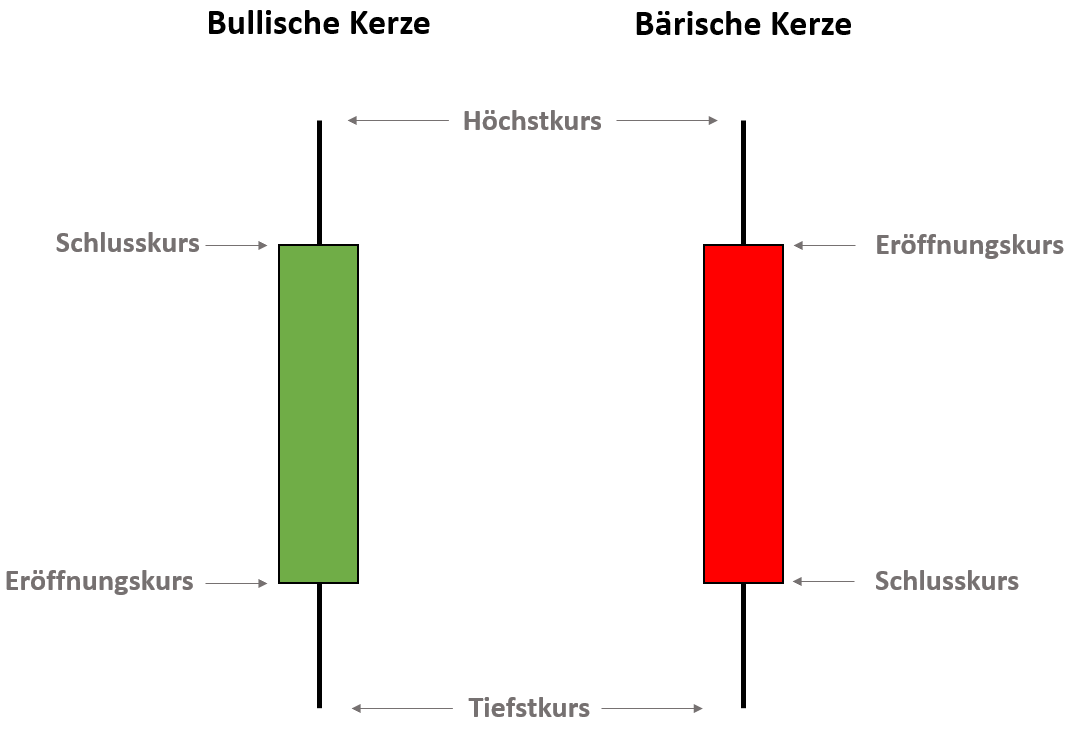
\includegraphics[height=0.45\textheight]{img/candles.png}
  \caption{Kerzen eines Candlestick Charts}
  \label{fig:1}
\end{figure}

Jede Kerze kann dabei für jede beliebige Zeitspanne stehen. Für
einen Tag, eine Woche, einen Monat, oder auch für kurzfristigere
Zeitebenen auf Minutenbasis. Die Aussagen der Kerzen sind dabei jedoch
immer dieselben.

Die Farbe der Candles lässt dabei sofort erkennen, ob es sich um eine
bullische, oder eine bärische Kerze handelt. Die \textbf{bullische
Kerze} symbolisiert ein Zeitintervall, welches positiv verlief, weil
der Schlusskurs über dem Eröffnungskurs des Intervalls lag. Analog
dazu bedeutet die \textbf{bärische Kerze}, dass der Kursverlauf
während des Zeitintervalls der Kerze negativ verlief, weil der
Schlusskurs unter dem Eröffnungskurs lag. Wichtig ist es dabei, sich
im Kopf zu behalten, dass jede Kerze immer nur eine Aussage über den
Kursverlauf ihres Zeitintervalls darstellt. (vgl.
\cite{candles_explained})
 
Fügt man alle Candles zu einem Candlestick Chart zusammen erhält man
ein Diagramm wie in Abbildung \ref{fig:2} dargestellt. \\

\begin{figure}[H]
  \centering
  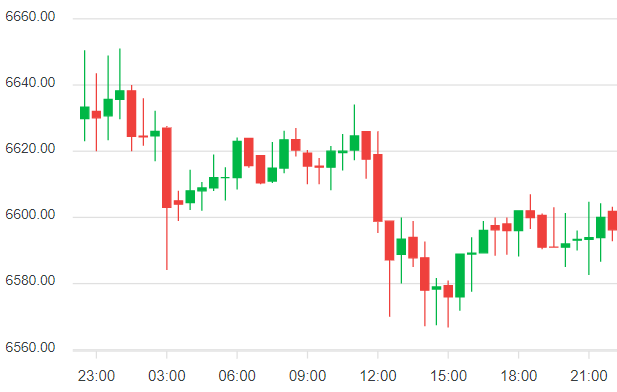
\includegraphics[height=0.43\textheight]{img/candlestick_chart.png}
  \caption{Beispiel eines Candlestick Chart\cite{candlestick_chart_pic}}
  \label{fig:2}
\end{figure}

\subsection{Technische Indikatoren}
\label{sub:technische_Indikatoren}

Technische Indikatoren sind Chart-Analyse-Tools, die Tradern helfen
können, Preisbewegungen besser zu verstehen und darauf zu reagieren.
Es gibt eine riesige Auswahl an technischen Analysewerkzeugen, die
Trends analysieren, Preisdurchschnitte liefern, die Volatilität
(Schwankung) messen und mehr. (vgl. \cite{technical_indicators})

Ein sehr beliebter technischer Indikator ist der \textbf{Moving
Average}, zu Deutsch: gleitender Mittelwert, welcher benutzt wird, um
den durchschnittlichen Schlusskurs des Marktes über einen bestimmten
Zeitraum darzustellen. Trader machen oft Gebrauch von Moving Averages,
da sie ein guter Hinweis auf die aktuelle Marktdynamik sein können.
(vgl. \cite{moving_average})

\textbf{Wie wird ein Moving Average berechnet?} \\
Eine der gängigsten Moving Averages ist der einfache gleitende
Mittelwert bzw. \ac{sma}, welche einfach der Durschnitt aller
Datenpunkte in der Serie geteilt durch die Anzahl der
Punkte\cite{moving_average}.

A = $ \{ $ {a$_{1}$, a$_{2}$, ..., a$_{n}$} $ \} $ \\
n = Number of time periods / price elements

SMA = $\frac{a_1 \ + \ a_2 \ + \ ... \ + \ a_n}{n}$

Betrachtet man zum Beispiel eine 5-Tage-SMA auf einem Tages-Chart von
EUR/USD und die Schlusskurse über die letzten 5 Tage sind wie folgt.

Tag 1: 1.321 \\
Tag 2: 1.301 \\
Tag 3: 1.325 \\
Tag 4: 1.327 \\
Tag 5: 1.326

SMA = (1.321 + 1.301 + 1.325 + 1.327 + 1.326)/5 = 1.32

Veranschaulichen lässt sich dieser Indikator gut in einem Candlestick
Chart, wie in Abbildung \ref{fig:3} dargestellt.

\begin{figure}[H]
  \centering
  \includegraphics[height=0.32\textheight]{img/sma.png}
  \caption{Simple Moving Average (in Gelb) innerhalb eines Candlestick Charts}
  \label{fig:3}
\end{figure} 

\subsection{Trading Strategien}
\label{sub:trading_strategien}

Eine Trading Strategie ist eine Methode zum Kaufen und Verkaufen auf
Märkten, die auf vordefinierten Regeln basiert, die zum Treffen von
Handelsentscheidungen verwendet werden\cite{trading_strategy}.

Es gibt viele Arten von Handelsstrategien, aber sie basieren
größtenteils entweder auf technischen Daten oder auf
Fundamentaldaten. Letzteres beschreibt langfristige, grundlegende
Informationen über die realen Produktionsmöglichkeiten, die
Strukturen der Wirtschaft sowie den Vermögensstatus der
Wirtschaftseinheiten, welche in dieser Arbeit jedoch nicht näher
betrachtet werden\cite{fundamentaldaten}. Die Gemeinsamkeit ist, dass
sich beide auf quantifizierbare Informationen stützen, die auf ihre
Genauigkeit hin rückgetestet werden können.
Technische Handelsstrategien verlassen sich auf technische
Indikatoren, um Handelssignale zu generieren. Technische Trader
glauben, dass alle Informationen über ein bestimmtes Wertpapier o.Ä.
in seinem Preis enthalten sind und dass er sich in Trends bewegt.
(vgl. \cite{trading_strategy}) 

Eine einfache Trading Strategie kann zum Beispiel eine
\textbf{Moving-Average-Strategy} sein, bei welcher ein Kaufsignal
erzeugt wird, sobald der aktuelle Preis einen gewissen Wert unter dem
der Moving Average liegt. Betrachtet man im Hinblick auf diese
Strategie noch einmal Abbildung \ref{fig:3}, lassen sich einige
Stellen im Chart erkennen, bei denen diese Strategie wohl Kaufsignale
erzeugen würde. 

%----

\section{Kryptowährungen}
\label{sec:kryptowährungen}

Eine Kryptowährung ist eine digitale oder virtuelle Währung, die
durch Kryptographie gesichert ist, was es nahezu unmöglich macht, sie
zu fälschen oder doppelt auszugeben. Viele Kryptowährungen sind
dezentralisierte Netzwerke, die auf der Blockchain-Technologie
basieren - einem verteilten Hauptbuch, das von einem verteilten
Netzwerk von Computern erzwungen wird. Ein entscheidendes Merkmal von
Kryptowährungen ist, dass sie im Allgemeinen nicht von einer
zentralen Behörde ausgegeben werden, was sie theoretisch immun gegen
staatliche Eingriffe oder Manipulationen macht.

Die erste Blockchain-basierte Kryptowährung war Bitcoin, die
immernoch die beliebteste und wertvollste ist. Heute gibt es tausende
von alternativen Kryptowährungen mit verschiedenen Funktionen und
Spezifikationen. Einige davon sind Klone oder Abspaltungen von Bicoin,
während andere neue Währungen sind, die von Grund auf neu entwickelt
wurden. (vgl. \cite{cryptocurrency_explained})

\subsection{Die Blockchain}
\label{sub:blockchain}

Einfach ausgedrückt ist eine Blockchain nichts anderes als eine
verteilte, öffentliche Datenbank\cite{blockchain_definition}, wessen
Funktionsprinzip die meisten Kryptowährungen zugrunde
liegen\cite{blockchain_1}.
Um das Prinzip einer Blockchain verstehen zu können, hilft der
Vergleich mit einem Gruppenchat:

Ben, Lisa und Mia haben sich um 14 Uhr im Park verabredet. Diese
Information ist nach dem Absenden auf allen Smartphones im Chatverlauf
gespeichert. Mia überlegt es sich anders und möchte sich erst um 16
Uhr treffen. Diese Entscheidung kann sie aber nicht alleine fällen.
Sie kann auch nicht einfach die Uhrzeit im Chatverlauf nachträglich
ändern. Mia muss also entweder gemeinsam mit den anderen von vorne
planen, oder sie steht um 16 Uhr alleine im Park. Niemand kann
nachträglich etwas verändern. Dieses Prinzip ist der Kern einer
Blockchain, denn auch hier werden Informationen in einem "Verlauf"
gespeichert. Informationen sind hierbei hauptsächlich
Transaktionsinformationen von Nutzern die diese getätigt haben.

Jede Information bildet einen Block, für welche ein Hash -
vergleichbar mit einem digitalen Fingerabdruck - berechnet wird.
Zusätzlich enthält dieser Hash, den Hash des vorherigen Blocks. So
werden die Blöcke über die Hashes, wie in Abbildung \ref{fig:4}
veranschaulicht, zu einer Kette verbunden. Ähnlich wie bei einem
Chatverlauf können die Informationen nicht verändert werden.
Verändert sich nämlich die Information, verändert sich auch der
Hash und die Kette würde auseinander brechen. Genau wie Mia und ihre
Freunde mit der Planung von vorne beginnen müssten, müssten die
Hashes aller folgenden Blöcke neu berechnet werden. (vgl.
\cite{blockchain})

\begin{figure}[H]
  \centering
  \includegraphics[height=0.16\textheight]{img/blockchain.png}
  \caption{Veranschaulichung einer Blockchain\cite{blockchain}}
  \label{fig:4}
\end{figure} 

Die Blockchain wird über ein dezentrales Netzwerk verwaltet, dem
jeder beitreten kann. Jedes Mitglied hat eine vollständige Kopie der
kompletten Blockchain auf dem Computer, welche von diesem auch
geprüft wird. Ein neuer Block wird erst hinzugefügt, wenn ihn jeder
im Netzwerk verifiziert hat. Jeder kontrolliert sozusagen jeden, was
die Blockchain damit sehr sicher macht. Wichtig ist dabei aber nicht
der Mensch vor dem Computer, oder eine dritte Instanz wie
beispielsweise ein Notar. Die Kontrolle, und somit das Vertrauen,
werden von der Blockchain technisch hergestellt. (vgl.
\cite{blockchain})

\subsection{Mining}
\label{sub:mining}

Wie das Geld herkömmlicher Währungen wie beispielsweise Euro oder
Dollar entsteht, ist kein Geheimnis. Das Bargeld entsteht unter
staatlicher Regie. Das Recht zur Prägung von Münzen liegt direkt
beim Staat, während die staatliche Bundesbank Scheine herstellt.
Beides müssen die privaten Geschäftsbanken bei der Bundesbank
kaufen. (vgl. \cite{herstellung_fiat_waehrung}). Doch wie funktioniert
dies bei Kryptowährungen?  

Instanzen einer Kryptowährung werden bei einem Prozess erzeugt, der
\textbf{Mining}, zu Deutsch: Bergbau, genannt wird. Diese Analogie ist
eigentlich recht passend, da neue Coins nur gefunden werden können,
wenn ein bestimmter Arbeitsaufwand betrieben wird.

Der vorrangige Sinn des Minings ist jedoch nicht die Erschaffung von
Coins, welcher eher als Nebeneffekt zu verstehen ist. Der Sinn des
Mining ist vor allem das Verifizieren und Durchführen von
Transaktionen sowie die Überprüfung, ob sich alle Teilnehmer des
Netzwerks an dessen Regeln halten. Der Prozess des Minings wird dabei
von Minern - also Computern mit Rechenleistung - durchgeführt. Wie
bereits in Unterkapitel \ref{sub:blockchain} beschrieben, enthalten
die Blöcke gewisse Transaktionsinformationen. Zustäzlich zu diesen
Transaktionsinformationen besitzt jeder Block eine \textbf{Coinbase
Transaktion}, welche neue Coins enthält, die dann als "Belohnung"
für das Sichern des Netzwerkes an die Miner ausgezahlt werden.  

Ein Miner versucht im Endeffekt also, Transaktionen zu einem Block zu
verbinden. Hat er diese Transaktionsinformationen zu einem passenden
Block verbunden, wird er der Blockchain hinzugefügt und der Miner
für seine Arbeistleistung bezahlt. Veranschaulichen lässt sich
dieser Prozess durch die Analogie eines Puzzles.  Hierbei versucht der
Miner, das Bild des Puzzles (Blockchain) zu bilden, indem er
Puzzlestücke (Blöcke) zusammenfügt. Wer das passende Puzzlestück
findet, erhält die Belohnung. (vgl. \cite{mining})


\subsection{Handel von Kryptowährungen}
\label{sub:handel_von_kryptowährungen}

Kryptowährungen werden in sogenannten \textbf{Wallets} gespeichert.
Das sind digitale Geldbörsen, die auf den unterschiedlichsten
digitalen Geräten wie beispielsweise einem Computer, Smartphone oder
USB-Stick liegen können. Anders als beim klassischen Geldsystem, wo
das Geld bei einer Bank und innerhalb eines Girokontos verwaltet wird,
gehören diese Wallets nur dem Besitzer, was bedeutet, dass niemand
diese Geldbörsen sperren kann. Auch viele andere Einschränkungen
normaler Wärhungen kennt eine Kryptowährung nicht. So gibt es
beispielsweise keine Überweisungslimits, maximale Transaktionshöhen
oder geografische Einschränkungen. Überweisungen können problemlos
von jedem Ort der Welt an jeden Ort der Welt gesendet werden, solange
Sender und Empfänger Internetzugang haben und ein Wallet besitzen.
(vgl. \cite{bitcoins_erklärung})

Wer sich nun dazu entschlossen hat mit Kryptowährungen zu handeln,
hat generell zwei Möglichkeiten:

\textbf{1. Bitcoins kaufen} \\
Der direkte Weg wäre Coins zu kaufen und diese solange zu halten, bis
der erwünschte Kursanstieg erreicht wurde, um sie dann wieder zu
verkaufen. Dazu wird jedoch, wie oben beschrieben, ein Wallet
benötigt. Die Coins werden dann auf Exchange Börsen oder
Krypto-Marktplätzen im Internet gekauft und an das eigene Wallet
geschickt.  

\textbf{2. Trading über CFDs} \\
Alternativ besteht die Möglichkeit des Crypto Trading per \ac{cfd}.
Hierbei spekulieren Anleger lediglich auf den Anstieg bzw. den Fall
des Bitcoin Kurses. Dabei können Basiswerte festegelegt werden, zu
denen die CFDs gekauft bzw. verkauft werden sollen. Steigt der Bitcoin
im Wert um 10\%, dann steigt auch der Wert der erworbenen CFDs um
10\%. (vgl. \cite{crypto_trading})

%----

\section{Application Programming Interface}
\label{sec:api}

Ein Application Programming Interface, bzw. Programmierschnittstelle,
ist ein Programmteil, der von einem Softwaresystem anderen Programmen
zur Anbindung an das System zur Verfügung gestellt wird. Die
Programmanbindung findet dabei auf Quelltext-Ebene statt. (vgl.
\cite{api_definition})

Ein Restaurant bildet ein System. Kunden wollen dieses System nutzen,
indem sie mithilfe einer Essenskarte Bestellungen aufgeben. Dabei ist
die Küche der Teil des Systems, der die Bestellungen der Gäste
zubereitet. Was fehlt, ist das entscheidende Bindeglied, um die
Bestellung der Kunden an die Küche zu übermitteln und ihnen ihr
Essen an den Tisch zu liefern. An dieser Stelle kommt der Kellner ins
Spiel. Der Kellner ist der Bote, bzw. \ac{api}, der die Anfrage der
Kunden entgegennimmt und der Küche - bzw. dem System - mitteilt, was
zu tun ist. Dann liefert der Kellner die Antwort an den Kunden
zurück. In diesem Fall ist es das Essen. (vgl. \cite{api_example})    

\subsection{REST API}
\label{sub:rest_api}
REST steht für Representational State Transfer und beschreibt ein
Paradigma (grunsätzliche Denkweise) für die Softwarearchitektur von
verteilten Systemen, insbesondere für Webservices. \ac{rest} ist eine
Abstraktion der Struktur und des Verhaltens des World Wide Web und hat
das Ziel, einen Architekturstil zu schaffen, der die Anforderungen des
moderen Web besser darstellt. Der Zweck von \ac{rest} liegt
schwerpunktmäßig auf der Kommunikation zwischen Client und Server in
Netzwerken. Eine \ac{rest} \ac{api} ist demnach also eine
Programmierschnittstelle die diesem Paradigma folgt. (vgl.
\cite{rest})

Die Funktionsweise wird in Abbildung \ref{fig:5} ersichtlich.

\begin{figure}[H]
  \centering
  \includegraphics[height=0.35\textheight]{img/rest_api.jpeg}
  \caption{Funktionsweise einer REST API\cite{rest_pic}}
  \label{fig:5}
\end{figure}

Die \ac{api} kommuniziert mit dem Server über das sogenannte
\ac{http} - ein Protokoll zur Übertragung von Daten über ein
Rechnernetz. Es wird hauptsächlich eingesetzt, um Websiten aus dem
World Wide Web in einen Webbrowser zu laden\cite{http_definition}.
Mittels \ac{http} Request, werden also Informationen vom Server
angefordert, wodurch der Server wiederum eine \ac{http} Response
erzeugt, die der Client dann erhält. Um eine Request an die
\ac{api} zu senden, werden \ac{url} benutzt - wie man sie aus der 
Verwendung eines Browsers kennt. Je nachdem, welche \ac{url} kontaktiert
wird, führt die \ac{api} unterschiedliche Aktionen aus, die 
unterschiedliche Antworten liefern.

\section{Python}
\label{sec:python}

Technisch gesehen ist Python eine interpretierte, objektorientierte
High-Level-Programmiersprache mit dynamischer Semantik. Ihre auf hoher
Ebene eingebauten Datenstrukturen, kombiniert mit dynamischer
Typisierung und dynamischer Bindung, machen sie sehr attraktiv für
die schnelle Anwendungsentwicklung sowie für den Einsatz als
Skript-Sprache, um bestehende Komponenten miteinander zu verbinden.
Die einfach, leicht zu erlernende Syntax von Python betont die
Lesbarkeit und reduziert somit die Kosten für die Programmwartung.
Python unterstützt Module und Pakete, was die Modularität der
Programme und die Wiederverwendung von Code fördert. Der
Python-Interpreter und die umfangreiche Standardbibliothek sind in
Quell- oder Binärform für alle wichtigen Plattformen kostenlos
erhältlich und können frei verteilt werden. 
(vgl.\cite{python_definition})

Ein Python-Programm wird vom Python-Interpreter ausgeführt. Dieser
stellt dabei eine umfangreiche Standardbibliothek bereit, die vom
Programm verwendet werden kann. Außerdem erlaubt es die Python API
einem externen C-Programm, den Interpreter zu verwenden oder zu
erweitern. Dargestellt in Abbildung \ref{fig:6}.

\begin{figure}[H]
  \centering
  \includegraphics[height=0.43\textheight]{img/python_konzept.png}
  \caption{Veranschaulichung der grundlegenden Konzepte\cite{python_konzepte}}
  \label{fig:6}
\end{figure}

\subsection{Pandas DataFrame}
\label{sub:dataframe}

\ac{pandas} ist ein beliebtes Python-Paket, das schnelle, flexible und ausdrucksstarke Datenstrukturen bereitstellt, um die Arbeit mit strukturierten (tabellarischen, mehrdimensionalen, potenziell heterogenen) Daten einfach und intuitiv zu gestalten. Es zielt darauf ab, ein grundlegender High-Level-Baustein für die praktische, reale Datenanalyse in Python zu sein. (vgl. \cite{pandas_definition})

Eine der wichtigsten, von pandas bereitgestellten, Datenstrukturen ist der \textbf{DataFrame}. Ein DataFrame ist eine zweidimensionale größenveränderliche, tabellarische Datenstruktur mit beschrifteten Achsen. Das bedeutet, die Daten sind tabellarisch in Zeilen und Spalten ausgerichtet, wie in Abbildung \ref{fig:8} dargestellt. (vgl. \cite{dataframe_example})

\begin{figure}[H]
  \centering
  \includegraphics[height=0.37\textheight]{img/dataframe_example.png}
  \caption{Beispiel eines DataFrame\cite{dataframe_example}}
  \label{fig:8}
\end{figure}
 

\subsection{Typing}
\label{sub:typing}

%----

\section{HTML}
\label{sec:html}

%----

\section{Versionierung}
\label{sec:versionierung}

\subsection{Git}
\label{sub:git}

\subsection{Gitflow}
\label{sub:gitflow}

%---------------------------------------------------
\chapter{Problemanalyse}
\label{cha:problemanalyse}

Wie bereits in Kapitel \ref{sec:problemstellung} grob beschrieben,
befasst sich das Projekt und die Arbeit in erster Linie damit, ein
algorithmisches Handelssystem zu entwerfen. Um dieses Problem angehen
zu können, muss es vorab in mehrere Teilprobleme gebrochen werden,
welche wiederum in noch kleinere Teilprobleme zerlegt werden. So wird
klar, wie an das Problem herangegangen werden muss, welche Komponenten
zu entwickeln sind und welche Abhängigkeiten zwischen diesen
bestehen.

%----

\section{Konzeption einer Schnittstelle für Handelsplattformen}
\label{sec:schnittstelle_handelsplatform}

Wer Kryptowährungen handeln will, benötigt dazu eine Plattform, auf
der Einkäufe und Verkäufe getätigt werden. Hat man sich dazu
entschlossen am Handel von Kryptowährungen teilzunehmen, erstellt man
sich dazu ein Konto bei einem der hunderten Crypto-Trading-Anbieter.
Einmal getan, loggt man sich auf der Homepage oder der App des
Anbieters ein und ist für den Handel von Kryptowährungen bereit. Im
Vergleich zum Handeln von Hand, benötigt das Trading-System jedoch
eine \ac{api}, an die es anknüpfen kann, um mögliche Aktionen der
Plattform tätigen zu können. Einige der Anbieter für Crypto-Trading
stellen kostenlose \ac{api}s für die Nutzung mittels Code bereit.

\subsection{Auswahl einer Handelsplattform}
\label{sub:auswahl_plattform}

Um sich für eine geeignete Plattform entscheiden zu können, bedarf
es mehr als die Bereitstellung einer funktionstüchtigen \ac{api}.
Nach welchen Kriterien sollte eine Handelsplattform also ausgewählt
werden? \\

\underline{Anforderungen an die Plattform:}
\begin{enumerate}
	\item \textbf{Gewährleistung der Sicherheit des Accounts} \\
		Die Sicherheit des Accounts und der damit 
		verbundene Wert, der aus dem Besitz von Kryptowährungs hervorgeht hat
		höchste Priorität. Eine Bereitstellung von Zwei-Faktor-Authentifizierung
		sollte daher gegeben sein.
	\item \textbf{Niedrige Transaktionsgebühren} \\
		Alle Plattformen verdienen einen Großteil ihres Umsatzes durch das
		Erheben von Transaktionsgebühren. Oft unterscheiden sich diese von
		Plattform zu Plattform. Ein Abwägen der Gebühren untereinander ist
		somit durchaus sinnvoll.
	\item \textbf{Handeln von Kryptowährungen gegen Fiatgeld} \\
		Das Handeln von Kryptowährungen gegen Fiatgeld (Euro, Dollar, usw.)
		ist von großem Vorteil. Denn so entfällt der oft mühsame Währungs-
		wechsel. Fehlt die Möglichkeit dazu, dann können Trader aussschließlich
		Kryptowährungen untereinander tauschen.
	\item \textbf{Breite Auswahl an verschiedenen Kryptowährungen} \\
		Eine breite Auswahl an handelbaren Kryptowährungen ist von großem
		Vorteil. Die Kurse verschiedener Kryptowährungen unterliegen
		unterschiedlich großen Schwankungen und manche Strategien funktionieren
		bei einigen Währungen besonders gut. \\
\end{enumerate}

\underline{Anforderungen an die \ac{api}:}
\begin{enumerate}
	\item \textbf{Geeignete Dokumentation der \ac{api}} \\
		Um später mit den von der \ac{api} bereitgestellten Funktionen arbeiten
		zu können, bedarf es einer guten und nutzerfreundlichen Dokumentation.
		Wird diese garnicht oder in nur sehr geringen Maße von der Plattform
		angeboten, gestaltet sich die Einbindung und Verwendung der 
		Funktionalitäten sehr schwierig und mühsam.
	\item \textbf{Bereitstellung von Marktdaten} \\
		Einer der wohl wichtigsten Anforderungen an eine \ac{api} für
		Crypto-Trading ist die Bereitstellung von Marktdaten. Dabei müssen nicht
		nur aktuelle Preisdaten zur Verfügung gestellt werden, sondern auch
		historische - also bereits verganene - Preisdaten bereitgestellt werden.
		Diese werden vor allem für den Backtest und die Verwendung von
		Strategien und deren Indikatoren benötigt. 
	\item \textbf{Bereitstellung von Symbolinformationen} \\
		Als Symbolinformationen bezeichnet man Informationen über die von der
		Handelsplattform angebotenen Symbole bzw. Kryptowährungen. Ein Symbol
		bezeichnet die Art des Handels und besteht dabei immer aus den Währungen
		zwischen denen gehandelt wird - also beispielsweise Bitcoin und Euro.
		Natürlich möchte man wissen, welche Symbole derzeit handelbar sind und
		welche Kaufoptionen für sie möglich sind.
	\item \textbf{Bereitstellung der Börsenhandelsregeln} \\
		Alle Handelsaktionen unterliegen Handelsregeln. Dabei unterscheidet man
		zwischen Handelsregeln für die Börse und den Handelsregeln eines
		bestimmten Symbols wie z.B. Mindestmenge und Maximalpreis.
	\item \textbf{Platzieren von verschiedenen Kaufaufträgen} \\
		Grundlegend muss es möglich sein, Käufe und Verkäufe platzieren zu
		können. Für zukünftige Zwecke werden jedoch die gängigen Order Types
		wie beispielsweise der Stop-Loss- oder Limit-Order benötigt. 
	\item \textbf{Bereitstellung von Accountdaten} \\
		Natürlich soll es außerdem möglich sein, Accountdaten per \ac{api}
		abfragen zu können. So können Daten wie z.B. derzeitiges Kapital, 
		offene Trades und viele andere Dinge dargestellt oder visualisiert
		werden.
\end{enumerate}

\subsection{Schnittstelle der API}
\label{sub:schnittstelle_der_api}

Eine von einer Plattform bereitgestellte \ac{api} reicht natürlich
nicht aus, um loslegen zu können. Vorerst muss sie sorgfältig in das
System eingebunden werden, das sie nutzen möchte. Dazu muss eine
weitere Schnittstelle entwickelt werden - sozusagen eine Schnittstelle
der Schnittstelle, um die Nutzung der \ac{api} einfacher zu gestalten.
Die Schwierigkeit liegt darin, die Schnittstelle möglichst generisch
und unkompliziert zu entwerfen. Es kann nämlich durchaus vorkommen,
dass sich eine andere Plattform als besser erweist als die Bisherige,
oder eine \ac{api} nicht länger unterstützt wird. Somit ist es
überaus wichtig, sicherzustellen, dass beim Austausch einer \ac{api}
so wenige andere Systemkomponenten beeinträchtigt werden wie
möglich.

%----

\section{Algorithmische Handelsstrategien und technische Indikatoren}
\label{sec:strategie_und_indikatoren}

Die richtige Trading Strategie entscheidet über Gewinn und Verlust
während technische Indikatoren die Werkzeuge jeder algorithmischen
Strategie sind. Somit stellen beide also eine enorm wichtige
Komponente des Systems dar. Wie bereits angedeutet, soll der Fokus
jedoch weniger auf der Findung und Konzeption neuer Strategien und
Indikatoren liegen, sondern darauf, wie diese möglichst einfach und
modular in das System eingebunden werden können. Ein Blick ins World
Wide Web genügt, um zu wissen, dass dort hunderte Kaufstrategien und
Indikatoren auf eine Implementierung in Code warten. Welche Strategie
davon nun die Beste ist, wird der Backtest früher oder später
herausfinden. Das ist jedoch nicht Teil dieser Arbeit.

Teil dieser Arbeit ist es aber, das System auf die parallele Nutzung
vieler Strategien und Indikatoren vorzubereiten, bzw. das System so zu
entwerfen, dass diese nach belieben ein- und ausgehängt werden
können. Das bedeutet, dass der Backtest beispielsweise in der Lage
sein soll, jede beliebige implementierte Strategie für seinen Test zu
Nutzen. Entscheidet man sich dazu, eine neue Strategie zu
implementieren, soll die Strategie (inklusive ihren Indikatoren) ins
System eingebunden werden können, ohne dabei die anderen Komponenten
des Systems zu verändern - also nahtlos. \\

\underline{Anforderungen an die technischen Indikatoren:}
\begin{enumerate}
	\item \textbf{Berechnen der Indikatordaten für gegebene Marktdaten} \\
		Jeder Indikator soll in der Lage sein, seine eigenen Indikatordaten
		auf der Basis gegebener Marktdaten zu berechnen. Bereitgestellt werden
		diese Daten durch die jeweilige Schnittstelle der Trading-Plattform-
		\ac{api}. 
	\item \textbf{Anhängen der Indikatordaten an die gegebenen Markdaten} \\
		Außerdem soll es möglich sein, die zuvor berechneten Indikatordaten an
		die Marktdaten anzuhängen, um somit ein Datenobjekt zu bilden, welches
		der jeweiligen Trading Strategie von Nutzen ist. \\
\end{enumerate}

\underline{Anforderungen an die Trading Strategie:}
\begin{enumerate}
	\item \textbf{Eigenständiges Hinzufügen der benötigten Indikatoren} \\
		Jede Strategie benötigt eine mehr oder weniger große Anzahl an
		Indikatoren, durch welche die Strategie in der Lage ist, Kaufs- und
		Verkaufsentscheidungen zu treffen. Jede Strategie sollte daher in der
		Lage sein, die benötigten Indikator-Instanzen selbst zu erzeugen und
		deren Daten anschließend an die Marktdaten anhängen zu lassen.
	\item \textbf{Überprüfen der Buy Condition} \\
		Die Buy Condition bezeichnet die Bedingung des Kaufes - also die
		Bedingung, die erfüllt sein muss, damit die Strategie einen Kauf für
		sinnvoll hält. Für die zukünftige Nutzung des Systems, soll die 
		Strategie also die Möglichkeit besitzen, Echtzeitdaten zu überprüfen 
		und für diese zu Entscheiden, ob ein Kauf platziert werden soll oder 
		nicht.
	\item \textbf{Erzeugung von Kaufsignalen} \\
		Ist die Buy Condition einer Strategie erfüllt, muss dem System ein Kauf
		signalisiert werden. Dies soll durch die Erzeugung von sogenannten Buy
		Signals erreicht werden, die dem System die zum Kauf benötigten 
		Informationen bereitstellen, womit dann ein Kauf platziert werden soll.
\end{enumerate}

%----

\section{Backtesting von Trading Strategien}
\label{sec:backtesting}

Der Backtest ist die wohl wichtigste Komponente des zu entwickelnden
Systems. Durch den Backtest soll der Nutzer in der Lage sein, eine
beliebige, im System implementierte, Trading Strategie auszuwählen
und auf Trading Symbole wie Bitcoin/Euro oder Ethereum/Euro laufen zu
lassen. Da der Backtest für seinen Rückvergleich sowohl die Trading
Strategie als auch die vergangenen Marktdaten benötigt, erfordert er
das Zusammenspiel der anderen Komponenten mit sich selbt. \\

\underline{Anforderungen an den Backtest:}
\begin{enumerate}
	\item \textbf{Durchführen des eigentlichen Backtest} \\
		Zur Durchführung des eigentlichen Backtests gehört das auswerten der 
		historischen Marktdaten. Es soll möglich sein, ein Startkapital
		festzulegen, mit welchem der Backtest startet. Anschließend soll ein
		Echtzeitszenario nachgeahmt werden, bei dem der Backtest chronologisch
		durch die historischen Marktdaten geht und ein Kaufen und Verkaufen von
		Kryptowährungs-Instanzen simuliert.  
	\item \textbf{Sammeln von Backtestdaten und Statistiken} \\
		Um erkennen zu können, ob die Strategie innerhalb des Zeitraums der 
		vergangenen Marktdaten Erfolg gehabt hätte, ist es wichtig, während des 
		Backtests eine Vielzahl	von Daten und Statistiken zu sammeln. So soll am
		Ende des Rückvergleichs beispielsweise ersichtlich werden, wie sich das
		Kapital entwickelt hat, wie viel Geld ausgegeben wurde und wie viel
		Gewinn die Strategie generiert hätte.
	\item \textbf{Bereitstellung der Backtestdaten} \\
		Die während des Backtests gesammelten Informationen sollen dem Nutzer
		in einem gut lesbaren Format ausgegeben werden. Damit soll ihm
		die Möglichkeit gegeben werden, die Effizienz der Strategie anhand der
		gesammelten Statistiken zu bewerten.
	\item \textbf{Visualisierung der Backtestdaten} \\
		Um dem Nutzer das Evaluieren der Backtest-Ergebnisse einfacher zu
		gestalten, sollen die historischen Marktdaten mithilfe eines
		Candlestick Charts visualisiert werden. Zusätzlich sollen auch die
		von der Strategie genutzten Indikatoren und die erzeugten Kauf- und
		Verkaufspunkte ersichtlich werden.
	\item \textbf{Speichern der Backtestdaten} \\
		Damit der Nutzer die Ergebnisse verschiedener Backtests auch noch in
		Zukunft auswerten und vergleichen kann, sollen die Backtest-Ergebnisse
		persistent gemacht werden.
\end{enumerate}

%----

\section{Entwurf und Verwaltung eines Trading Bots}
\label{sec:trading_bot}

Da innerhalb dieser Arbeit nur das Fundament für die Erstellung und
Verwaltung von Trading Bots gelegt werden soll, wird der Trading Bot
nicht in der Lage sein, eigenständig Einkäufe und Verkäufe zu
tätigen. Vielmehr soll ein Konzept erarbeitet werden, das die
Erstellung und Nutzung dieser Trading Bots in das System integriert.
Die zukünftige Implementierung des Features für reale Käufe und
Verkäufe soll dann auf diesem Konzept aufbauen. \\

\underline{Anforderungen an den Trading Bot}
\begin{enumerate}
	\item \textbf{Sammeln der nötigen Marktdaten} \\
		Damit ein Trading Bot Anwendung findet, benötigt er einen Datensatz aus
		Echtzeitdaten. Daher soll er in der Lage sein, nach der Instanzierung
		eines neuen Bots, eigenständig die richtigen Marktdaten zu sammeln und zu
		verwalten.
	\item \textbf{Updaten der Marktdaten} \\
		Um die Marktdaten aktuell zu halten, muss der Trading Bot die Möglichkeit
		haben, seinen Datensatz selbständig zu aktualisieren.
	\item \textbf{Evaluierung von Echtzeitdaten} \\
		Der Bot soll zudem in der Lage sein, diesen Ständig aktualisierten
		Marktdatensatz auszuwerten, um die Empfehlung eines Kaufes oder Verkaufes
		zu signalisieren. \\
\end{enumerate}

\underline{Anforderungen an die Verwaltung des Trading Bots}
\begin{enumerate}
	\item \textbf{Hinzufügen und Entfernen neuer Trading Bots} \\
		Die Verwaltungskomponente soll sowohl in der Lage sein alle Trading Bots 
		zu verwalten, als auch neue zur Verwaltung hinzuzufügen.
	\item \textbf{Starten und Stoppen der Trading Bots} \\
		Analog zum Hinzufügen neuer Trading Bots, soll außerdem eine Möglichkeit 
		zum Entfernen von Trading Bots gegeben sein. \\
\end{enumerate}

Da der Trading Bot für die oben genannten Anforderungen sowohl
Marktdaten als auch Trading Strategie zur Auswertung benötigt, muss
eine reibungslose Zusammenarbeit mit den anderen Systemkomponenten
gewährleistet sein.

%----

\section{Erstellung einer Konsolenanwendung}
\label{sec:erstellung_cli}

Alle bereits aufgeführten Komponenten und Features sollen Teil einer
Konsolenanwendung werden, welche diese dann als System vereint und dem
Nutzer zur Interaktion bereitstellt. \\

\underline{Anforderungen an die Konsolenanwendung}
\begin{enumerate}
	\item \textbf{Erstellen eines Backtests} \\
		Die Erstellung eines Backtests soll dem Nutzer so einfach wie möglich
		gemacht werden. Der Nutzer soll daher eine Konfiguration des Backtests
		durchlaufen, indem er die verschiedenen Parameter wie Tradingsymbol oder 
		Strategie, auswählt.
	\item \textbf{Erstellen eines neuen Trading Bots} \\
		Die Erstellung eines neuen Trading Bots soll ähnlich ablaufen wie die des
		Backtests. Auch hier soll der Nutzer eine Konfigurationsauswahl
		durchlaufen.
	\item \textbf{Anzeigen der erstellten Trading Bots} \\
		Sind erstmal ein paar Trading Bots erstellt, ist es natürlich von Vorteil
		sich diese Anzeigen zu lassen. Daher soll die Möglichkeit gegeben sein,
		alle vom System verwalteten Trading Bots aufzulisten und deren aktuellen
		Status anzuzeigen.
	\item \textbf{Beenden des Programms} \\
		Ein beenden des Programms von der Konsolenanwendung aus soll ebenfalls
		bereitgestellt werden.
	\item \textbf{Einfache und intuitive Bedienung} \\
		Einer der wichtigsten Aspekte einer Benutzeroberfläche ist deren
		Bedienbarkeit. Kein Nutzer möchte sich bei der Nutzung eines Programms
		"verloren" fühlen und sich andauern fragen wie etwas funktioniert. Die
		Konsolenanwendung muss daher so gestaltet werden, dass sich auch Nutzer
		ohne Entwicklungshintergrund zurechtfinden.
	\item \textbf{Übersichtliches und konsistentes Designkonzept} \\
		Die Übersichtlichkeit und damit verbundene Konsistenz eines Designs 
		innerhalb der Anwendung sind entscheidende Faktoren im Bereich 
		Benutzerfreundlichkeit und sollten daher durchaus berücksichtigt werden.
\end{enumerate}

%----

\section{Zusammenfassung}
\label{sec:zsmf_komponenten}

Die nachfolgende Abbildung (Abb. \ref{fig:7}) dient der
Veranschaulichung der zu entwickelnden Komponenten und deren
Abhängigkeiten untereinander.

\begin{figure}[H]
  \centering
  \includegraphics[height=0.45\textheight]{img/components.png}
  \caption{Veranschaulichung der grundlegenden Komponenten}
  \label{fig:7}
\end{figure}

\underline{Erklärung der Abhängigkeiten:}
\begin{itemize}
	\item Sowohl Trading Bot als auch der Backtest sollen die Schnittstelle der
		\ac{api} verwenden, um von dort aus die nötigen Marktdaten zu beziehen.
	\item Zusätzlich sollen Trading Bot und Backtest die im System
		zu implementierenden Trading Strategien nutzen, um damit deren gesammelten 
		Marktdaten auszuwerten.
	\item Technische Indikatoren sind Bestandteil jeder Trading Strategie und
		sollen der Analyse von Marktdaten dienen.
	\item Instanzen eines Trading Bots sollen von einem Verwaltungssytem gehalten,
		gestartet und gestoppt werden.
\end{itemize}

%---------------------------------------------------
\chapter{Lösungskonzept}
\label{cha:loesungskonzept}

%----

\section{Schnittstelle für Handelsplattformen}
\label{sec:schnittstelle_für_handelsplattformen}

\subsection{Auswahl einer Handelsplattform}
\label{sub:auswahl_einer_handelsplattform}

Bevor mit der Konzeption einer Schnittstelle für eine Handelsplattform begonnen werden kann, muss sich für eine der vielen Plattformen entschieden werden. Diese Entscheidung fiel auf die Verwendung der Crypto-Trading-Plattform \textbf{Binance}. Die Plattform bietet den Handel von hunderten, verschiedenen Kryptowährungen an, welche auch gegen Fiatgeld gehandelt werden können. Zum Zeitpunkt dieser Arbeit berechnet Binance eine durchschnittliche Gebühr von etwa 0,1\% auf jeden Trade, den ein Benutzer tätigt. Obwohl die Plattform keine genauen Angaben darüber bereitstellt, wie die Gelder gesichtert werden, wird Binance für eine sichere Plattform gehalten. Zwei-Faktor-Authentifizierung wird unterstützt. (vgl. \cite{binance})

Die von Binance bereitgestellte \ac{rest} \ac{api} ist, der Menge der im Internet bereitgestellten Lernressourcen nach, eine der verbreitetsten \ac{api}s unter algorithmischen Tradern. Zu ihr gibt es eine Vielzahl an Tutorials und eine ausgesprochen gute Dokumentation, welche auf GitHub unter folgendem Link zur Verfügung steht: \url{https://github.com/binance/binance-spot-api-docs/blob/master/rest-api.md}

\subsection{Entwurf einer Schnittstelle}
\label{sub:entwurf_einer_schnittstelle}

Wie bereits angedeutet erfolgt die Kommunikation mit Binance über eine \ac{rest} \ac{api}. Das bedeutet, um an die Daten der Plattform zu kommen, müssen \ac{url}s erzeugt werden, mit deren Hilfe die sogenannten \textbf{Endpoints} kontaktiert werden. Jeder Endpoint erwartet eine unterschiedliche Menge an Parametern, die ebenso per \ac{url} übergeben werden müssen.

Die Aufgabe der Schnittstelle ist es dabei, den oben genannten Prozess innerhalb ihrer Methoden zu verstecken und wiederverwendbar zu machen. Das bedeutet, dass die anderen Komponenten des Systems nicht wissen müssen, wie die verschiedenen Endpunkte zu kontaktieren sind und wie sie deren Antworten verarbeiten müssen. Dargestellt wird dieses Konzept in Abbildung \ref{fig:9}

\begin{figure}[H]
  \centering
  \includegraphics[height=0.34\textheight]{img/binance_interface_konzept.png}
  \caption{Konzept der REST API Schnittstelle}
  \label{fig:9}
\end{figure}

\textbf{Beispiel 1:} \\
Der Backtest benötigt eine Menge an Candlestick Daten, an welche er theoretisch über die von Binance bereitgestellte \ac{rest} \ac{api} kommt. Dennoch tätigt der Backtest den \ac{api}-Call nicht selbst, sondern lässt dies das Binance Interface für sich erledigen. Das bedeutet, der Backtest benötigt keinerlei Informationen darüber, wie er die \ac{api} für die benötigten Daten kontaktieren muss, sondern erhält sie einfach über die Binance Schnittstelle.

\textbf{Beispiel 2:} \\
Nun benötigt auch ein Trading Bot eine Menge an Candlestick Daten um seinen Echtzeit-Datensatz an Marktdaten zu initialisieren. Auch er muss nicht wissen, wie er an die Daten kommt, sondern lässt sie sich, ebenso wie der Backtest, von der Schnittstelle geben. Somit werden Arbeitsschritte voneinander getrennt und ebenso Code-Redundanz vermieden.

Um eine einfache Weiterverarbeitung der Candlestick Daten zu gewährleisten, sollen die Daten in die, im Kapitel \ref{sub:dataframe} beschriebene, Datenstruktur \textbf{DataFrame} eingepflegt werden und an die anderen Komponenten zurückgegeben werden.

%----

\section{Technische Indikatoren}
\label{sec:technische_Indikatoren}

Der technische Indikator dient der Strategie zur Analyse der Marktdaten. Damit diese der Strategie jedoch zur Verfügung stehen, muss die Möglichkeit bestehen, die Indikatordaten eines jeden Indikators auf gegebene Marktdaten zu berechnen und sie anschließend an diese anzuhängen. Somit genügt ein einfacher Erweiterungsprozess der Marktdaten um die vom Indikator berechneten Daten, um die Datengrundlage einer jeden Trading Strategie zu bilden. Daraus ergibt sich folgender Entwurf (Abbildung \ref{fig:10})

\begin{figure}[H]
  \centering
  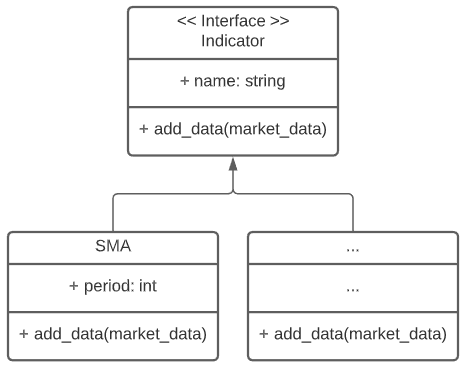
\includegraphics[height=0.34\textheight]{uml/indicators_uml.png}
  \caption{Einfache Darstellung der Indikatoren durch ein Klassendiagramm}
  \label{fig:10}
\end{figure}

Durch die Definition eines Interface wird gewährleistet, dass jede neu hinzugefügte Klasse, die von der Klasse \textit{Indicator} erbt, dazu verpflichtet ist, alle innerhalb des Interface definierten Methoden zu überschreiben. Damit wird erreicht, dass jeder Indikator das gleiche Funktionsprinzip hat und ein einheitliches Konzept bei der Implementierung verwendet wird.

Jeder Indikator-Instanz wird ein Name übergeben, welcher durch die Zuweisung an das Attribut \textit{name} der eindeutigen Identifikation eines Indikators dient. Zusätzlich sind alle Indikatoren dazu verpflichtet, eine Methode \textit{add\_data(market\_data)} zu implementieren, welche die indikatorspezifischen Daten an die übergebenen Marktdaten anhängt und zurückgegeben.

Im Rahmen dieser Arbeit wird soll nur ein Indikator implementiert und verwendet werden - der \textbf{Simple Moving Average}, welcher bereits im Grundlagenkapitel \ref{sub:technische_Indikatoren} beschrieben wurde.

%----

\section{Algorithmische Trading Strategien}
\label{sec:algorithmische_trading_strategien}

Eine gute Trading Strategie ist beim algorithmischen Traden der Schlüssel zum Erfolg, denn sie entscheidet darüber, ob ein Kauf platziert werden soll oder nicht. Wie sinnvoll dieser Kauf ist, obliegt der Entscheidung des Traders, welcher die Strategie implementiert. Damit im weiteren Verlauf des Projekts weitere, vermutlich bessere Strategien eingebunden werden können, ist der Entwurf eines guten Konzepts dafür von großer Wichtigkeit.

\subsection{Einbindung von Trading Strategien}
\label{sub:einbindung_von_trading_strategien}

Da jede Strategie eine gewisse Anzahl an bereitgestellten Funktionen bieten muss, macht die Nutzung eines Interfaces auch hier Sinn. Daraus folgt ein, zu den Indikatoren ähnlicher Entwurf, dargestellt in Abbildung \ref{fig:11}

\begin{figure}[H]
  \centering
  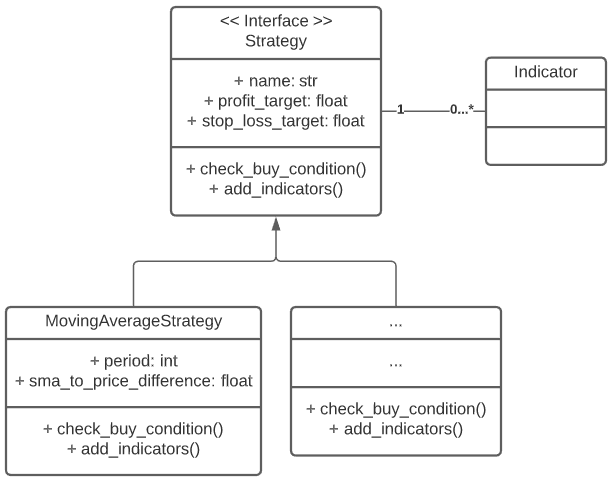
\includegraphics[height=0.45\textheight]{uml/strategy_uml.png}
  \caption{Einfache Darstellung von Strategien durch ein Klassendiagramm}
  \label{fig:11}
\end{figure}

Wie aus dem Klassendiagramm ersichtlich wird, benötigt jede Strategie die Instanz-Attribute \textit{name}, \textit{profit\_target} und \textit{stop\_loss\_target}. Letztere Beiden werden zum Setzen von Stop-Loss Preisen im Backtest benötigt - mehr dazu im darauf folgenden Kapitel. Jede Strategie kann eine Vielzahl an verschiedener Indikatoren besitzen, welche die Strategie zur Analyse der Daten herbeizieht (aus Gründen der Übersichtlichkeit hier als leere Klasse dargestellt). Jede neue implementierte Strategie erbt die Eigenschaften des Interface \textit{Strategy} und verpflichtet sich damit, die im Interface definierten Methoden zu implementieren. \textit{check\_buy\_condition()} wird dazu benötigt, die Buy Condition zu überprüfen, welche die Strategie ausmacht. Da jede Strategie selbst entscheiden soll, welche Indikatoren sie zur Analyse der Daten benötigt, soll sie durch die Methode \textit{add\_indicators()} in der Lage sein, diese den Daten selbstständig hinzuzufügen.

Welche Strategie innerhalb dieses Projekts verwendet werden soll, lässt sich durch einen Blick auf das Klassendiagramm in Abbildung \ref{fig:11} vermuten. Ebenso wie der verwendete Indikator, wurde auch die \textbf{Moving Average Strategie} bereits im Grundlagenkapitel \ref{sub:trading_strategien} beschrieben.

%----

\section{Backtest}
\label{sec:backtest}

\subsection{Entwurf eines Backtests}
\label{sub:entwurf_eines_backtests}

Der Entwurf eines geeigneten Backtest stellt die wohl wichtigste Aufgabe dieses Kapitels dar und sollte gut durchdacht sein. Er steht in direkter Verbindung zu den bereits beschriebenen Klassen \textit{Binance} und \textit{Strategy}. Zusätzlich werden drei neue Klassen benötigt, um den Ablauf des Backtests möglich nah am Ablauf des realen Trading zu halten. In der nachfolgenden Abbildung (Abb. \ref{fig:12}) wird dieses Konzept in vereinfachter Form dargestellt. Das heißt, es wurden im Hinblick auf die Übersichtlichkeit der Darstellung nur die wirklich für den Backtest benötigten Methoden und Attribute dargestellt.

\begin{figure}[H]
  \centering
  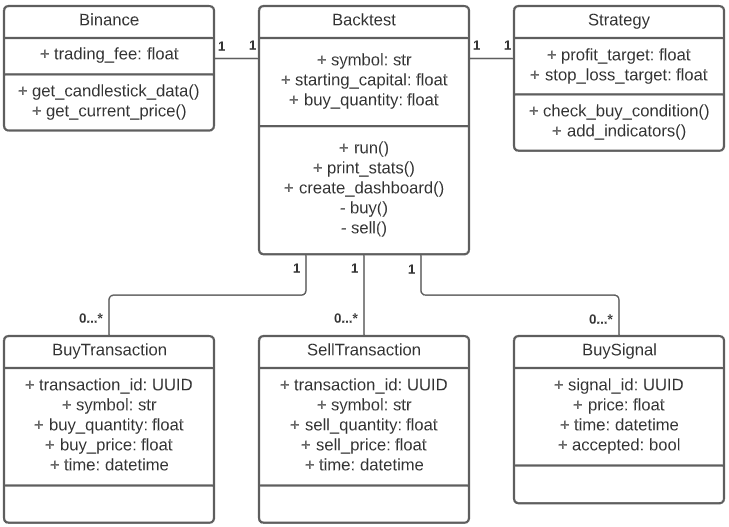
\includegraphics[height=0.48\textheight]{uml/backtest_uml.png}
  \caption{Vereinfachte Darstellung der Klasse \textit{Backtest} innerhalb eines 		Klassendiagramms}
  \label{fig:12}
\end{figure}

Jeder Backtest benötigt eine \ac{api} \textit{Binance}, von der er die benötigten Marktdaten abrufen kann. Diese Marktdaten müssen innerhalb des Backtests mit der Hilfe einer \textit{Strategy} verarbeitet werden. Um einen Kauf zu simulieren, benötigt der Backtest ein \textit{BuySignal} welches ihm signalisiert, dass die Buy Condition der gewählten Strategie getroffen wurde. Die Klassen \textit{BuyTransaction} und \textit{SellTransaction} werden benötigt, um einen Kauf bzw. Verkauf zu simulieren und werden trotz ihrer Ähnlichkeit als zwei getrennte Klassen definiert, da die Nutzung einer einzelnen Transaktionsklasse innerhalb des Backtests schnell zur Verwirrung führen kann.

\subsection{Funktionsweise des Backtest}
\label{sub:funktionsweise_des_backtest}

Interessant ist vor allem die Methode \textit{run}, da sie für den automatischen Ablauf des Backtests zuständig ist und alle anderen Komponenten des Backtests und der oben definierten Klassen verwendet. Veranschaulicht wurde dieser Ablauf in Abbildung \ref{fig:13}.

\begin{figure}[H]
  \centering
  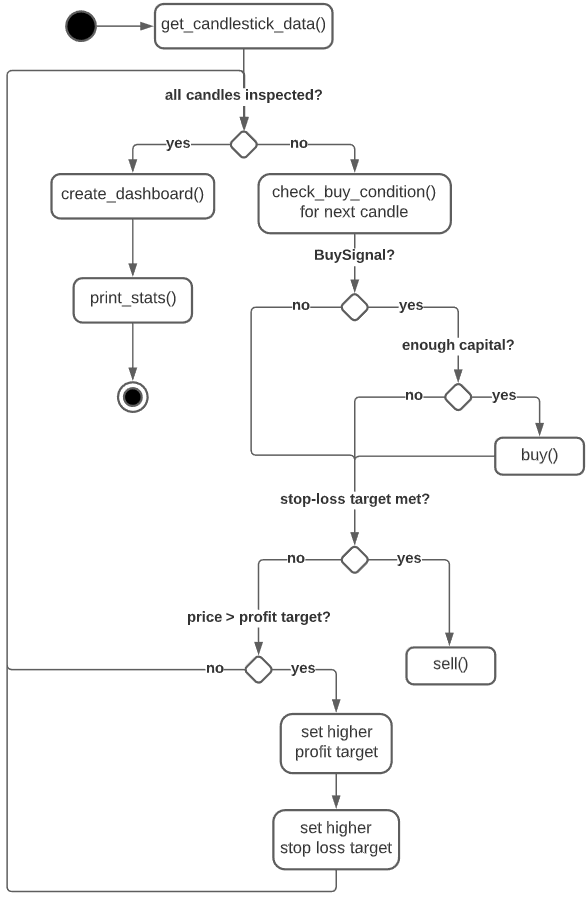
\includegraphics[height=1\textheight]{uml/backtest_activity_uml.png}
  \caption{Aktivitätsdiagramm für den Ablauf eines Backtest}
  \label{fig:13}
\end{figure}

\textbf{get\_candlestick\_data()} \\
Zu beginn des eigentlichen Backtest wird die Schnittstelle \textit{Binance} dazu beauftragt Candlestick Daten von der \ac{rest} \ac{api} zu sammeln und in einem DataFrame zurück zu liefern. Dieser soll nun Candle für Candle analysiert werden.

\textbf{check\_buy\_condition()} \\
Für jede Candle lassen wir die gewählte Strategie ihre Buy Condition überprüfen. Erhält der Backtest ein \textit{BuySignal} für die aktuelle Candle, wird überprüft, ob überhaupt genügend Kapital vorhanden ist, um einen Kauf zu platzieren.

\textbf{buy()} \\
Ist das für den Kauf benötigte Kapital vorhanden, platzieren wir einen Kauf. Innerhalb dessen soll die entsprechende \textit{BuyTransaction} generiert und dem Backtest hinzugefügt werden. Nun sollte überprüft werden, ob der Preis das festgelegte \textit{stop\_loss\_target} erreicht hat, welches ein Verkaufen von allen besessenen Coins bedeutet.

\textbf{sell()} \\
Analog für jede \textit{BuyTransaction} soll nun eine \textit{SellTransaction} generiert werden, welche einen symbolischen Kauf darstellt. Somit werden bei erreichen des Stop-Loss Target alle bisher gehaltenen Coins verkauft.

\textbf{set higher profit target / set higher stop loss target} \\
Da wir einen Coin möglichst so lange halten möchten wie er profitabel ist, überprüft der Backtest nun, ob der Preis der aktuellen Candle das festgelegte \textit{profit\_target} überschritten hat. Ist dies der Fall, legen wir höhere Werte für beide Variablen fest.

\textbf{create\_dashboard()} \\
Wurden alle Candles und damit die gesamten Marktdaten untersucht, wird ein Dashboard generiert, welches dem Nutzer eine Visualisierung der Marktdaten bietet. 

\textbf{print\_stats()} \\
Während des gesamten Backtest werden verschiedene Daten zur Erhebung einer Statistik gesammelt, die dem Nutzer zeigt, wie erfolgreich der Backtest für eine gewählte Strategie und das gewählte Symbol ist.

\subsection{Visualisieren des Backtests}
\label{sub:visualisieren_des_backtests}

Für die Erstellung eines Candlestick Chart o.Ä. gibt es eine Vielzahl von Python Libraries, welche enorme Unterstützung bieten und einem den Großteil der eigentlichen Arbeit abnehmen. Die dabei verwendete Library nennt sich \textit{plotly} und stellt nützliche Methoden für die Visualisierung von Finanzdaten bereit. Die erzeugten Diagramme lassen sich als \ac{html} abspeichern und im Browser öffnen. Da jedoch noch andere Daten mit in das Dashboard einfließen sollen, sollen mehrere \ac{html} Objekte erzeugt und zu einer Datei zusammengefügt werden. Der Ablauf ist dabei wie in Abbildung \ref{fig:18} dargestellt.

\begin{figure}[H]
  \centering
  \includegraphics[height=0.52\textheight]{img/dashboard_creation.png}
  \caption{Erstellungsvorgang eines Dashboards}
  \label{fig:18}
\end{figure}

\begin{enumerate}
	\item \textbf{Erstellung eines Candlestick Charts als HTML Objekt:} \\
		Mithilfe der Library \textit{plotly} wird ein Candestick Diagramm in Form
		eines HTLM Objekts erzeugt und bis zur Weiterverarbeitung verwahrt.
	\item \textbf{Erstellung eines Diagramm zur Visualisierung des Kapitals:} \\
		Innerhalb des Backtests wird bei jedem Kauf und Verkauf eine Veränderung
		des Kapitals zu diesem genauen Zeitpunkt der Transaktion gespeichert.
		Somit ist es möglich, das Kapital im zeitlichen Rahmen des Backtests als
		Liniendiagramm darzustellen. Dieses soll ebenfalls mithilfe von
		\textit{plotly}, in Form eines HTML Objekts, erzeugt und verwahrt werden.
	\item \textbf{Umwandlung der Backtest Statistiken in HTML Code:} \\
		Auch die beim Backtest generierten Statistikdaten sollen in das Dashboard
		eingebaut werden. Diese müssen mithilfe von Variablen-Substitution in
		vorbereiteten HTML Code eingefügt werden.
	\item \textbf{Erzeugen des Dashboards:} \\
		Sind alle Objekte erzeugt, müssen diese noch zu einem großen Objekt
		zusammengefügt und zu einer Datei verarbeitet werden. Bei der Speicherung
		des \ac{html} Dashboards wird gleichzeitig eine geeignete Ordnerstruktur
		erzeugt.
\end{enumerate}

%----

\section{Entwurf und Verwaltung eines Trading Bot}
\label{sec:schnittstelle_für_handelsplattformen}

Wie bereits erwähnt, wird im Rahmen dieser Arbeit kein funktionstüchtiger Trading Bot entworfen, sondern lediglich dessen Fundament und Integration im Trading System - dargestellt in Abbildung \ref{fig:14}.

\begin{figure}[H]
  \centering
  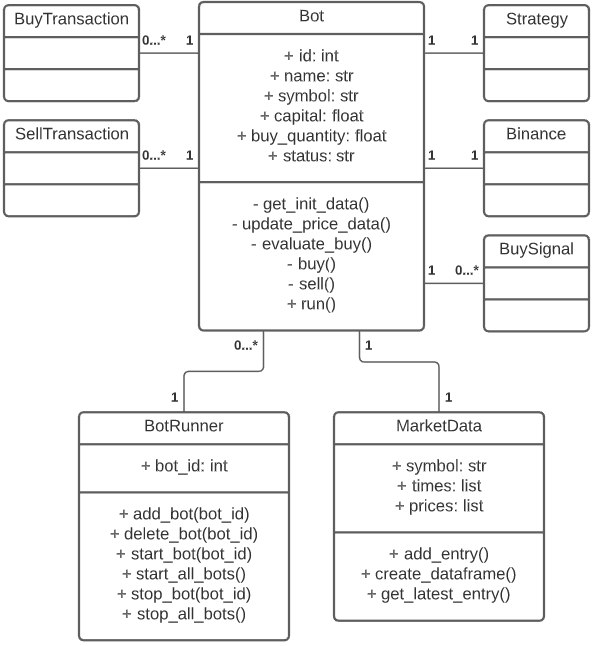
\includegraphics[height=0.65\textheight]{uml/bot_uml.png}
  \caption{Konzept eines Trading Bot und dessen Verwaltung als UML Diagramm}
  \label{fig:14}
\end{figure}

Ähnlich wie auch der Backtest, nutzt der Trading Bot nahezu alle anderen Komponenten des Systems. Die Schnittstelle \textit{Binance} versorgt ihn mit Marktdaten, während die Strategie zur Auswertung dieser dient. Wird ein BuySignal erzeugt, entscheidet das Kapital über einen Kauf bzw. die Erstellung einer BuyTransaction. Analog dazu entscheidet das Stop-Loss Target der Strategie über einen Kauf bzw. die Erstellung einer SellTransaction.

Bisher unbekannt sind die Klassen \textit{BotRunner} und \textit{MarketData}. Die MarketData Klasse bildet ein Objekt aus Marktdaten, welches unter ständiger Verwaltung und Modifikation des Bots steht, da es eine feste Größe an beinhaltenden Daten hat und durchgehend aktuell gehalten werden muss.

Der BotRunner dient der Verwaltung aller Bots. Nach Erzeugung eines jeden Bots durch den Nutzer, wird dieser dem BotRunner hinzugefügt. Der BotRunner soll in der Lage sein, entweder alle oder einen einzelnen Bot zu starten oder zu stoppen. Somit bildet er zusammen mit der Konsolenanwendung die "höchste" \ Komponente des Systems.

%----

\section{Entwurf einer Konsolenanwendung}
\label{sec:entwurf_einer_konsolenanwendung}

\subsection{User Interface}
\label{sub:user_interface}

Das User Interface ist das, was der User sieht, wenn er die Konsolenanwendung startet. Durch dieses ist er in der Lage, mit dem System zu interagieren und bestimmte Aktionen ausführen zu lassen. Das User Interface sollte sich möglichst intuitiv gestaltet werden um dem Nutzer eine einfache Nutzung zu bieten. Daher sollte auch das Designkonzept konsistent angewendet worden. Aus den bereits ermittelten Anforderungen ergibt sich das nachfolgende Designkonzept (Abb. \ref{fig:15}).

\begin{figure}[H]
  \centering
  \includegraphics[height=0.43\textheight]{img/cli_mockup.png}
  \caption{User Interface der Konsolenanwendung}
  \label{fig:15}
\end{figure}

Bei jeder Aktion die der Nutzer tätigen kann, soll ein dementsprechender Header angezeigt werden, der die gewählte Aktion beschreibt. So soll beim Starten der Anwendung beispielsweise ein Willkommens-Banner angezeigt werden, während beim Erstellen eines neuen Backtest der entsprechende Backtest-Header gezeigt werden soll.

Die Interaktion mit dem User soll hauptsächlich durch die Auswahl von Optionen geschehen. Dadurch wird der User bei den verschiedenen Aktion an die Hand genommen und ihm immer alle möglichen Aktionen aufgezeigt. Startet er z.B. die Anwendung, soll der Nutzer gefragt werden, was er tun möchte. Zur Auswahl stehen die zur Verfügung stehenden Features, aus denen er wählen kann, indem er die korrespondierende Zahl eingibt.

\subsection{Zusammenspiel mit anderen Komponenten}
\label{sub:zusammenspiel_mit_anderen_komponenten}

%----

Über das User Interface steuert der Nutzer alle großen Komponenten des Systems, welche durch den BotRunner, unter dem Dach der Konsolenanwendung, miteinander vereint werden (dargestellt in Abbildung \ref{fig:15}). Backtest und Bot werden beide vom \textit{CommandLineInterface} erstellt und im Falle des \textit{Bot} and den \textit{BotRunner} zur Verwaltung weitergereicht.

\begin{figure}[H]
  \centering
  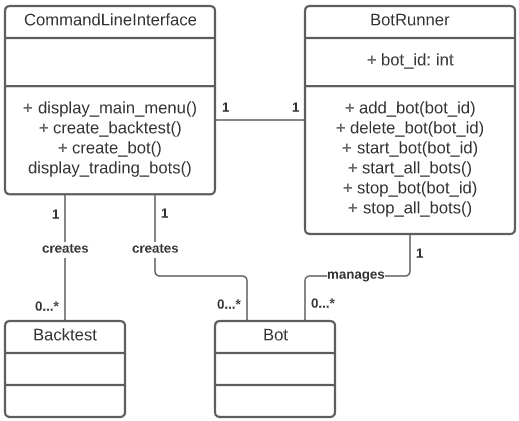
\includegraphics[height=0.42\textheight]{uml/cli_uml.png}
  \caption{Die Konsolenanwendung dargestellt als Klassendiagramm}
  \label{fig:15}
\end{figure}

%---------------------------------------------------
\chapter{Implementierung}
\label{cha:implementierung}

bla bla bla was über python implementierung sagen als einleitung

%----

\section{Binance Schnittstelle}
\label{sec:binance_schnittstelle}

\subsection{Vorgehen}
\label{sub:vorgehen}

Im Prinzip sind alle Datenbeschaffungsfunktionen der Klasse \textit{Binance} Implementierungen ähnlicher Manier. Das bedeutet, jede Methode, deren Aufgabe die Beschaffung eines gewissen Datensatzes, wie beispielsweise Preisdaten oder Symbolinformationen, folgt der gleichen Vorgehensweise und besteht immer aus den folgenden Schritten:

\begin{enumerate}
	\item Erstellen der URL für den jeweiligen Endpoint der REST API
	\item Senden einer HTTP Request an die erstellte URL
	\item Überprüfung der empfangenen HTTP Response
	\item Überführung der Daten in eine geeignete Form oder Datenstruktur
\end{enumerate}

\subsection{Klassendefinition}
\label{sub:klassendefinition}

Die Schnittstelle der Binance \ac{api} wurde innerhalb einer Python File mit dem Namen \textit{binance.py} implementiert. Hier wurde zunächst eine Klasse \textit{Binance} definiert:

\lstset{language=Python}
\lstset{frame=lines}
\lstset{caption={Binance Klassendefinition}}
\lstset{label={lst:binance_constructor}}
\lstset{basicstyle=\footnotesize}
\textbf{binance.py}
\begin{lstlisting}
class Binance:
	# Symbols
    SYMBOL_BITCOIN_EURO = "BTCEUR"
    SYMBOL_ETHEREUM_EURO = "ETHEUR"
    SYMBOL_LITECOIN_EURO = "LTCEUR"

	# Endpoints
    ENDPOINT_KLINES = "/api/v3/klines"
    ENDPOINT_PRICE = "/api/v3/ticker/price"
    ENDPOINT_TIME = "/api/v3/time"
    ENDPOINT_TEST_ORDER = "/api/v3/order/test"
    ENDPOINT_EXCHANGE_INFO = "/api/v3/exchangeInfo"
	
	# Constructor
	def __init__(self):
		self.base = "https://api.binance.com"
		self.trading_fee = Binance.TRADING_FEE
\end{lstlisting}

Bevor die Klasse durch den Konstruktor instanziiert werden kann, werden mehrere Klassenvariablen definiert: \\
\begin{itemize}
	\item \textbf{Symbols (Zeile 3-5):} \\
		Zunächst werden die für diese Arbeit verfügbaren Trading Symbole
		festgelegt. Jedes Symbol stellt die zwei Währungen dar, zwischen denen
		gehandelt werden soll.
	\item \textbf{Endpoints (Zeile 8-12):} \\
		Als nächstes werden die verschiedenen Endpunkte der \ac{rest} \ac{api}
		definiert, welche benötigt werden um die gewollten Informationen
		anzufragen.
	\item \textbf{Konstruktor (Zeile 15-17):} \\
		Anschließend wird ein Konstruktor implementiert, welcher die Klasse 
		instanziiert. Dort werden die beiden Instanzvariablen \textit{base} 
		(\ac{url} der \ac{rest} \ac{api}) und \textit{trading\_fee} (Prozentsatz 
		der Trading-Gebühren) festgelegt. 	

\end{itemize}
\subsection{API Anfragen}
\label{sub:api_anfragen}

Bevor die Beschaffung der Marktdaten o.Ä. betrachtet werden kann, muss verstanden werden, wie eine Anfrage an die \ac{api} der Trading-Plattform Binance gehandhabt wird.

\lstset{language=Python}
\lstset{frame=lines}
\lstset{caption={Binance API Calls}}
\lstset{label={lst:api_calls}}
\lstset{basicstyle=\footnotesize}
\textbf{binance.py}
\begin{lstlisting}
def http_request(self, endpoint, params=None):
	# Create URL
	url: str = self.base + endpoint
	if params:
		for i in range(len(params)):
			if i == 0:
				# First param has to connect with a question mark to the url
				url = url + "?" + params[i]
			else:
				# Other params connect with a ampersand
				url = url + "&" + params[i]
\end{lstlisting}

Eine \ac{url} wird erzeugt, indem man die \textit{base} mit dem jeweiligen \textit{endpoint} verbindet. Jede \ac{url} kann das Verhalten der \ac{api} durch eine Mitgabe an Parametern modifizieren. Parameter werden, wie der Endpoint, beim Aufruf der Methode an Übergeben. Bei den Parametern geschieht dies über den optionalen Übergabewert \textit{params}. 

Ob Parameter übergeben werden oder nicht, wird in Zeile 4 abgefragt. Wenn ja, muss der erste Parameter mit einem \textbf{?} an die \ac{url} gehängt werden, während alle weiteren Parameter mit einem \textbf{\&} hinzugefügt werden. So entsteht beispielsweise folgedende \ac{url}: https://api.binance.com/api/v3/ticker/price?symbol=LTCEUR

\lstset{language=Python}
\lstset{frame=lines}
\lstset{caption={Binance API Calls Fortsetzung}}
\lstset{label={lst:code_direct}}
\lstset{basicstyle=\footnotesize}
\textbf{binance.py}
\begin{lstlisting}
# Call url to get excepted response
try:
	response: Response = requests.get(url)
except requests.exceptions.ConnectionError as e:
	logger.error(f"ConnectionError: {e}")
	return False

# Check response
try:
	response.raise_for_status()
except requests.exceptions.HTTPError as e:
	logger.error(f"HTTP error: {e}")
	return False

# Decode data
try:
	data = response.json()
except JSONDecodeError as e:
	logger.error(f"Could not decode data from {url}: {e}")
	return False
else:
	return data
\end{lstlisting}

Nachdem die \ac{url} des gewollten Endpoints erzeugt wurde, werden die Daten nun abgefragt, überprüft und verarbeitet:
\begin{itemize}
	\item \textbf{API Aufruf (Zeile 2-6):}
		Um das Arbeiten mit \ac{http} Anfragen möglichst einfach zu gestalten
		wird das Package \textit{requests} verwendet. Es wird eine GET Anfrage mit
		der erzeugten URL gestartet, durch welche die API eine HTTP-Response
		erzeugt, welche im besten Fall die gefragten Daten beinhalten.
		Sollte während der Anfrage ein Verbindungsfehler auftreten, wird dieser
		Abgefangen und auf dem Terminal ausgegeben. Anschließend gibt die Methode
		\textit{False} zurück, um dem Aufrufer zu signalisieren, dass etwas falsch
		gelaufen ist.
	\item \textbf{Verarbeiten der HTTP Response (Zeile 9-13):} \\
		Trat kein Verbindungsfehler auf, untersuchen wir die HTTP Request nun auf
		seinen Status-Code. Dieser gibt Auskunft darüber, ob alles geklappt hat,
		oder Fehler aufgetreten sind. Wird ein fehlerhafter Status-Code entdeckt,
		wird ein Fehler erzeugt, welcher in gleicher Manier abgefangen wird wie
		zuvor der Verbindungfehler.
	\item \textbf{Dekodieren der Daten (Zeile 16-22):} \\
		Da die Daten einem textbasiertem Format namens \ac{json} von der API an 
		den Aufrufer zurückgegeben werden, müssen diese vor Verwendung noch 
		dekodiert werden. Dabei werden die in der Response enthaltenen Daten
		durch das Package \textit{json} automatisch dekodiert. Tritt dabei ein
		Fehler auf, wird der Fehler wie bereits bekannt abgefangen und 
		\textit{False} zurückgegeben. Läuft alles wie es soll, werden die Daten
		in einer geeigneten Datenstruktur zurückgegeben.
\end{itemize}

\subsection{Sammeln von Candlestick Daten}
\label{sub:sammeln_von_candlestick_daten}

Eine der wichtigsten Funktionen der Binance Schnittstelle ist das Sammeln von Candlestick Daten, welche sowohl im Backtest als auch beim Initialisieren des Trading Bots benötigt werden.

Um dieser Anforderung Genüge zu tun, wurde eine Klassenmethode \textit{get\_candlestick\_data()} implementiert, welche eine festgelegte Menge an Candles für ein bestimmtes Trading Symbol von der \ac{api} anfordert und verarbeitet.

\lstset{language=Python}
\lstset{frame=lines}
\lstset{caption={Sammeln von Candlestick Daten}}
\lstset{label={lst:candlestick_data}}
\lstset{basicstyle=\footnotesize}
\textbf{binance.py}
\begin{lstlisting}
def get_candlestick_data(self, symbol, interval="1h", end_time=None, limit=1000):
	# Get data
	params = [
		"symbol=" + symbol,
		"interval=" + interval,
		"limit=" + str(limit)
	]
	if end_time:
		params.append("endTime=" + str(end_time))
	data = self.http_request(endpoint=self.ENDPOINT_KLINES, params=params)
	if not data:
		logger.error("Missing candlestick data")
		return False
\end{lstlisting}

Erklärung der Übergabeparameter:
\begin{itemize}
	\item \textbf{symbol:} \\
		Das Symbol bzw. die Währungen, für welche die Candlestick Daten angefragt
		werden.
	\item \textbf{intverval="1h":} \\
		Dieser optionale Parameter legt das Zeitintervall fest, welches die 
		angefragten Kerzen haben sollen. Diese gibt es beispielsweise in Minuten, 
		Stunden, Tagen und noch mehr. Wird kein Wert für den Parameter übergeben, 
		wird ein Standardwert von einer Stunde pro Intervall festgelegt.
	\item \textbf{end\_time=None:} \\
		Ein ebenfalls optionaler Parameter, welcher eine Zeit festlegt, von
		welchem aus die Daten (rückwärtsgehend) geholt werden soll. Wird kein
		Wert übergeben, werden einfach die neuesten Kerzen geholt.
	\item \textbf{limit=1000:} \\
		Das Limit legt fest, wie viele Kerzen abgefragt werden sollen. Dieses wird
		von Binance festgelegt und beträgt standardmäßig 500, maximal jedoch 1000.
\end{itemize}

In Zeile 2-10 werden die für die Candlestick Daten benötigten Parameter festgelegt, woraufhin anschließend die Daten geholt werden. Gab es während des Datenbeschaffungsprozess ein Problem, erhalten wir den boolschen Wert \textit{false}. Daher überprüfen wir in Zeile 11, ob beim Beschaffen der Daten alles geklappt hat. Sollte dies nicht der Fall sein, wird der Fehler auch in dieser Methode geloggt und \textit{False} zurückgegeben. Erhalten wir jedoch die gewollten Daten, liegen diese nun in folgendem Format vor: \\

\lstset{language=Python}
\lstset{frame=lines}
\lstset{caption={Candlestick Daten in Rohform}}
\lstset{label={lst:rohe_candlestick_daten}}
\lstset{basicstyle=\footnotesize}
\begin{lstlisting}
[
  [
    1499040000000,      // Open time
    "0.01634790",       // Open
    "0.80000000",       // High
    "0.01575800",       // Low
    "0.01577100",       // Close
    "148976.11427815",  // Volume
    1499644799999,      // Close time
    "2434.19055334",    // Quote asset volume
    308,                // Number of trades
    "1756.87402397",    // Taker buy base asset volume
    "28.46694368",      // Taker buy quote asset volume
    "17928899.62484339" // Ignore.
  ],
  [
  	...
  	...
  	...
  ],
  ...
]
\end{lstlisting}

Die hier abgebildete Datenstruktur \textit{list} enthält alle Candles in Form von weiteren Lists. Sozusagen ein zweidimensionales Array. Innerhalb jeder Candle befinden sich die oben erkennbaren Daten wie \textit{Open time} und \textit{Open}. Diese sollen nun für eine bessere Weiterverarbeitung in die Datenstruktur DataFrame eingepflegt werden: \\

\lstset{language=Python}
\lstset{frame=lines}
\lstset{caption={Sammeln von Candlestick Daten Fortsetzung}}
\lstset{label={lst:Daten der Kerzen in "Rohform"}}
\lstset{basicstyle=\footnotesize}
\textbf{binance.py}
\begin{lstlisting}
df = DataFrame(data)
df = df.drop(range(6, 12), axis=1)
col_names = ["time", "open", "high", "low", "close", "volume"]
df.columns = col_names

# Transform values from strings to floats
for col in col_names:
	df[col] = df[col].astype(float)
return df
\end{lstlisting}

Erklärung des restlichen Code:
\begin{itemize}
	\item \textbf{Erstellen eines DataFrame (Zeile 1-4:)} \\
		Das DataFrame Objekt wird erzeugt, indem man ihm die Candlestick Daten in
		der bereits vorliegenden Form einer Liste/Array übergibt. Anschließend
		werden die letzten sechs Spalten (beginnend bei "Close time")entfernt, da
		diese für die hier vorliegenden Zwecke nicht benötigt werden.
	\item \textbf{Transformieren der Textwerte in Gleitkommawerte (Zeile 7-8):} \\
		Um die in den Kerzen enthaltenen Werte Zahlenwerte für arithmetische
		Dinge nutzen zu können, müssen sie vorerst in Gleitkommawerte umgewandelt
		werden.	Anschließend wird der DataFrame an den Aufrufer der Methode
		zurückgegeben.	
\end{itemize}

Jede Zeile des DataFrame stellt nun eine Kerze, inklusive ihren korrespondierenden Daten dar. Abbildung \ref{fig:16} zeigt einen solchen DataFrame und mehrere dieser Kerzen.

\begin{figure}[H]
  \centering
  \includegraphics[height=0.5\textheight]{img/candlestick_df.png}
  \caption{Candlestick Daten innerhalb eines DataFrame}
  \label{fig:16}
\end{figure}

%----

\section{Indikatoren}
\label{sec:indikatoren}

\subsection{Abstrakte Basisklasse Indicator}
\label{sub:abstrakte_basisklasse_indikator}

Interfaces werden in Python anders gehandhabt als in den meisten anderen Sprachen und können in ihrer Designkomplexität variieren. Klassische Interfaces, wie man sie aus Sprachen wie Java oder C++ kennt, existieren in Python nicht. Daher wird auf die Verwendung einer Python Library mit dem Namen \ac{abc} verwendet. Durch dies ist man in der Lage, definierte Methoden als \textit{abstract} zu deklarieren, was den gewünschten Effekt eines Interfaces erzielt.

Da die Basisklasse der Indikatoren keine wirkliche Funktionalität enthält, besitzt sie eine simple Implementierung, dargestellt im nachfolgenden Code-Ausschnitt:

\lstset{language=Python}
\lstset{frame=lines}
\lstset{caption={Implementierung der abstrakten Basisklasse \textit{Indicator}}}
\lstset{label={lst:baseclass_indicator}}
\lstset{basicstyle=\footnotesize}
\textbf{indicators.py}
\begin{lstlisting}
from abc import ABC, abstractmethod

class Indicator(ABC):
    def __init__(self, name: str) -> None:
        self.name: str = name

    @abstractmethod
    def add_data(self, data: DataFrame, column_name: str):
        # Needs to be overridden in every subclass
        raise NotImplementedError("Missing implementation: Please override this method in the subclass")
\end{lstlisting}

Durch das Erben von der Klasse \textit{ABC} in Zeile 3 wird die Verwendung der Library \ac{abc} ersichtlich. Anschließend wird in Zeile 4-5 ein Konstruktor erzeugt, welche einen Indikator mit einem Namen instanziiert.

Der wichtigere Teil befindet sich in Zeile 7-10. Wie bereits in Kapitel \ref{sec:technische_Indikatoren} beschrieben, soll jeder Indikator dazu verpflichtet sein, die Methode \textit{add\_data} zu implementieren. Dies wird erreicht, indem über der Methodendeklaration ein sogenannter Decorator \textit{@abstractmethod} platziert wird (Zeile 7). Um dem Entwickler neuer Indikatoren ein Fehlverhalten im Falle einer Nicht-Implementierung mitzuteilen, erschaffen wir einen \textit{NotImplementedError} in Zeile 10. Wird nun ein neuer Indikator implementiert, die Methode \textit{add\_data} jedoch nicht überschrieben, erhebt das System einen Laufzeitfehler.

\subsection{Simple Moving Average}
\label{sub:simple_moving_average}

Für viele technische Indikatoren gibt es bereits bereitgestellte Implementierungen, welche durch die Verwendung von Packages in das System integriert werden können. Auch wenn diese als bereits fertige Objekte importiert werden können, soll die klare Struktur der Indikatoren beibehalten werden. Daher wird zunächst die Klasse \textit{SimpleMovingAverage} definiert:

\lstset{language=Python}
\lstset{frame=lines}
\lstset{caption={Klassendefinition SimpleMovingAverage}}
\lstset{label={lst:baseclass_indicator}}
\lstset{basicstyle=\footnotesize}
\textbf{indicators.py}
\begin{lstlisting}
from pyti.smoothed_moving_average import smoothed_moving_average as sma

class SimpleMovingAverage(Indicator):

    def __init__(self, name, period):
        super().__init__(name)  # Init parent class
        self.period: int = period
\end{lstlisting}

Durch das Erben von der Klasse \textit{Indicator} in Zeile 3, wird die Verwendung der zuvor definierten abstrakten Basisklasse deklariert. Im Konstruktor in Zeile 5-7 wird die Instanzvariable der Basisklasse (name) sowie die Instanzvariable period initialisiert.

Der wichtige Teil passiert jedoch in der Implementierung der nun überschriebenen Methode \textit{add\_data}:

\lstset{language=Python}
\lstset{frame=lines}
\lstset{caption={Implementierung der Methode \textit{add\_data}}}
\lstset{label={lst:baseclass_indicator}}
\lstset{basicstyle=\footnotesize}
\textbf{indicators.py}
\begin{lstlisting}
def add_data(self, data, column_name):
	calc_column = data[column_name].tolist()
	sma = sma(calc_column, self.period)
	data[self.name] = sma
	return data
\end{lstlisting}

Beim Aufruf der Methode werden zwei Übergabeparameter erwartet:
\begin{itemize}
	\item \textbf{data}: Der (Candlestick) DataFrame an welchen die Indikatordaten
		angehängt werden sollen.
	\item \textbf{colum\_name}: Der Name der Spalte, auf wessen Datengrundlage der
		Indikator berechnet werden soll.
\end{itemize}

Zunächst werden die Daten der Spalte, auf wessen Grundlage der Indikator berechnet werden soll, aus dem DataFrame extrahiert und zu einer Liste, bestehend aus diesen Werten, transformiert (Zeile 2). Anschließend wird unter der Verwendung dieser Daten sowie der festgelegten Periode ein SimpleMovingAverage erzeugt (Zeile 3). Am Ende werden die erzeugten Daten an den DataFrame in Form einer neuen Spalte angehängt und zurückgegeben.

Da man sich dieses Prinzip ohne ein wenig Übung im Umgang mit den genannten Datenstrukturen vielleicht schwer vorstellen kann, folgt ein visuelles Beispiel in Abbildung \ref{fig:17}). In diesem Beispiel wird der Simple Moving Average Indikator für gegebene Candlestick Daten berechnet und an diese angehängt.

\begin{figure}[H]
  \centering
  \includegraphics[height=0.7\textheight]{img/add_indicator_data.png}
  \caption{Berechnen und Hinzufuegen des SMA Indikator an einen DataFrame}
  \label{fig:17}
\end{figure}

%----

\section{Moving Average Strategie}
\label{sec:moving_average_strategie}

Die eigentliche Implementierung der Moving Average Strategie ist recht simpel. Da die Verwendung einer abstrakten Basisklasse schon im vorangegangenen Kapitel aufgezeigt wurde, wird diese Information hier weggelassen. Zunächst wird die Klasse definiert und ein paar wichtige Instanzvariablen initialisiert:

\lstset{language=Python}
\lstset{frame=lines}
\lstset{caption={Klassendefinition der Moving Average Strategy}}
\lstset{label={lst:}}
\lstset{basicstyle=\footnotesize}
\textbf{indicators.py}
\begin{lstlisting}
class MovingAverageStrategy(Strategy):

	def __init__(self):
		self.name = "Moving Average Strategy"
		self.profit_target = 1.05
		self.stop_loss_target = 0.85
		self.sma_to_price_difference = 1.03
		self.indicators = list()
\end{lstlisting}

Erklärung der Instanzvariablen:
\begin{itemize}
	\item \textbf{name}: Name der Strategie
	\item \textbf{profit\_target}: Das Profit Ziel liegt bei 5\% Preiszuwachs
	\item \textbf{stop\_loss\_target}: Das Stop-Loss Target liegt bei 15\% unter
		dem Kaufpreis. Wird dieser Preis erreicht, wird verkauft.
	\item \textbf{sma\_to\_price\_difference}: Liegt der Preis 3\% unter dem Wert
		des Simple Moving Average, soll gekauft werden
	\item \textbf{indicators}: Liste der von der Strategie verwendeten Indikatoren
\end{itemize}

Die Methoden der Strategie sind sehr einfach gehalten. Die Überprüfung der Daten zur Bestimmung eines Kaufes oder Nicht-Kaufes wird in gerade einmal 4 Zeilen Code erreicht:

\lstset{language=Python}
\lstset{frame=lines}
\lstset{caption={Klassendefinition der Moving Average Strategy}}
\lstset{label={lst:}}
\lstset{basicstyle=\footnotesize}
\textbf{indicators.py}
\begin{lstlisting}
    def check_buy_condition(self, price, time, row=None):
		sma = getattr(row, "slow_sma")

		# Check if we meet our strategy condition
		if sma > self.sma_to_price_difference * price:
			return BuySignal(price, time)
		else:
			return False
\end{lstlisting}

In Zeile 5 wird überprüft, ob der Wert des SMA drei Prozent über dem zugehörigen Preis liegt. Ist dies der Fall, wird ein \textit{BuySignal} erzeugt und zurückgegeben, ansonsten \textit{False}.

Das automatische Hinzufügen von Indikatoren läuft ebenfalls sehr simpel ab. Dabei werden die jeweiligen benötigten Indikatoren instanziiert und deren \textit{add\_data()} Funktion verwendet, um dem DataFrame die Indikatordaten hinzuzufügen. Anschließend werden alle Indikatorinstanzen zur Liste der Indikatoren (\textit{indicators}) hinzugefügt.

%----

\section{Backtest}
\label{sec:backtest}

Dass der Backtest die bisher komplexeste Komponente des Systems ist, spiegelt sich in seiner Implementierung wieder. Implementiert wurde der Backtest innerhalb der Datei \textit{backtest.py} welche mit über 400 Zeilen Code die größte Sourcefile darstellt.

\subsection{Ablauf des Backtests}
\label{sub:ablauf_des_backtests}

Das Herzstück des Backtests ist seine \textit{run()} Methode. Diese definiert den kompletten Ablauf des Backtests, welcher in Abbildung \ref{fig:13} durch ein Aktivitätenprogramm grob beschrieben wird. Der Übersichtlichkeit zuliebe werden nur Ausschnitte in vereinfachter Form gezeigt:

\lstset{language=Python}
\lstset{frame=lines}
\lstset{caption={Vereinfachte Darstellung der Methode \textit{run()}}}
\lstset{label={lst:}}
\lstset{basicstyle=\footnotesize}
\textbf{backtest.py}
\begin{lstlisting}
profit_target_price = -1
stop_loss_price = -1
for index, candle in candlestick_data_frame.iterrows():
	# Get close price and time of current candle
	close_price = getattr(candle, "close")
	time = getattr(candle, "time")
	buy_signal = strategy.check_buy_condition(close_price, time, candle)
	
	# Check whether we can buy
	if buy_signal:
		if capital >= close_price:
			buy(buy_signal)
			
			# We now have coins -> init targets
			profit_target_price = close_price * strategy.profit_target
			stop_loss_price = close_price * strategy.stop_loss_target
			
	# Check wheter we can sell
	if kept_coins:
		low_price: getattr(candle, "low")
		
		# Check whether stop-loss price was reached
		if low_price <= stop_loss_price:
			sell(stop_loss_price)  # sell all coins for sl price
			profit_target_price = -1  # reset
			stop_loss_price = -1  # reset
			
		# Check whether we need to set new targets
		elif close_price >= profit_target_price != -1:
			profit_target_price = close_price * strategy.profit_target
			stop_loss_price = close_price * strategy.stop_loss_target

# Create dashboard		
create_folder_structure()
create_candlestick_figure()
figures_to_html()
stats_to_html()
create_html_dashboard()
print_stats()
\end{lstlisting}

Beim Ablauf des Backtests muss jede einzelne Kerze auf einen Kauf oder Verkauf überprüft werden. Für jede Kerze werden der Close Price und dessen korrespondierende Zeit ermittelt (\textbf{Zeile 5-6}). Diese werden nun der Strategie übergeben, welche überprüft, ob gekauft werden soll oder nicht (\textbf{Zeile 7}). Wurde ein \textit{BuySignal} erzeugt, wird mithilfe von diesem ein Kauf simuliert (\textbf{Zeile 10-12}). Mithilfe des Preises, zu welchem gerade Coins erworben wurden, werden nun das Profitziel und der Stop-Loss gesetzt (\textbf{Zeile 15-16}).

Befinden sich nun Instanzen einer Kryptowährung im Besitz, muss auch für jede Kerze überprüft werden, ob der niedrigste Preis innerhalb ihres Zeitintervalls den definierten Stop-Loss Preis erreicht hat (\textbf{Zeile 19-23}). Ist dies der Fall, werden alle besessenen Coins verkauft und \textit{profit\_target\_price} sowie \textit{stop\_loss\_price} zurückgesetzt (\textbf{Zeile 24-26}).

Am Ende der Schleife wird überprüft, ob der Close Preis der aktuellen Kerze das definierte Profit-Ziel überschritten hat. Ist dies der Fall, werden \textit{profit\_target\_price} sowie \textit{stop\_loss\_price} neu gesetzt, um den möglichen Gewinn eines Kaufes zu maximieren (\textbf{Zeile 30-32}).

Als letztes werden innerhalb des Backtests implementierte Methoden zur Erzeugung eines HTML Dashboards aufgerufen und die im Backtest gesammelten Statistiken auf der Konsole ausgegeben (\textbf{Zeile 35-40}). 

\subsection{Erstellung eines Dashboards}
\label{sub:erstellung_eines_dashboards}

Unter der Verwendung der Bibliothek \textit{plotly} ergibt sich die Erstellung eines Finanzdiagramms als kein großes Hindernis. Für die Erstellung eines Candlestick Charts gibt es speziell dafür vorgefertigte Klassen, denen die Daten überreicht werden müssen:

\lstset{language=Python}
\lstset{frame=lines}
\lstset{caption={Erzeugung eines Candlestick Chart}}
\lstset{label={lst:}}
\lstset{basicstyle=\footnotesize}
\textbf{binance.py}
\begin{lstlisting}
def create_candlestick_figure(self):
	df = self.candlestick_df
	
	# Plot candlestick chart
	candle = Candlestick(
		x=df["time"],
		open=df["open"],
		close=df["close"],
		high=df["high"],
		low=df["low"],
		name="Candlesticks"
	)
	data = [candle]
	
	# Loop through all indicators of the market data and plot them
	for indicator in self.strategy.indicators:
		if type(indicator) == SimpleMovingAverage:
			sma = Scatter(
				x=df["time"],
				y=df[indicator.name],
				name=indicator.name,
				line=dict(color="rgba(255, 207, 102, 1)")
			)
			data.append(sma)
			
	# Customize style and display
	layout = Layout(
		xaxis={
			"title": self.symbol,
			"rangeslider": {"visible": True},
			"type": "date"
		},
		yaxis={
			"fixedrange": False,
			"title": "Price per coin"
		}
	)
	
	# Create figure and plot it
	figure = Figure(data=data, layout=layout)
	return figure
\end{lstlisting}

Erklärungen zum Code:

\begin{enumerate}
	\item \textbf{Erzeugen des Candles (Zeile 5-13:} \\
		Mithilfe der \textit{plotly} Library wird ein Candlestick Objekt erzeugt,
		dem die jeweiligen Daten, übergeben werden. Anschließend wird das Candle
		Objekt in eine Liste eingefügt, welche alle Daten des Diagramms enthält.
	\item \textbf{Erzeugen der Indikatoren (Zeile 16-24):} \\
		Für jeden Indikator den die gewählte Strategie besitzt, wird ein 
		sogenannter Scatter-Plot erzeugt, mit welchem sich Linien und Punkte
		darstellen lassen. Ihm werden die jeweiligen Zeiten und Indikatorwerte
		übergeben.
	\item \textbf{Festlegen eines Layouts (Zeile 27-41):} \\
		Bevor die erstellten Objekte in eine \textit{Figure} überführt werden
		können, welche die Objekte zu einem Diagramm vereint, kann ein Layout
		festegelegt werden. Mithilfe des Layouts können beispielsweise Titel und
		Achsenbeschriftungen angepasst werden.
\end{enumerate}

Die Erstellung des Diagramms zur Visualisierung des Kapitals lehnt sich stark an die oben gezeigte Erstellung des Candlestick Charts an. Die Substitution der Statistik Daten in den vordefinierten HTML Code läuft jedoch anders ab.

Zunächst wird eine HTML Datei definiert, welche die Darstellung der Daten vorgibt.
Mit dem nachfolgenden HTML Code kann eine Darstellung wie in Abbildung \ref{fig:19} erreicht werden:

\lstset{language=HTML}
\lstset{frame=lines}
\lstset{caption={HTML Vorlage}}
\lstset{label={lst:}}
\lstset{basicstyle=\footnotesize}
\textbf{binance.py}
\begin{lstlisting}
</p>
<hr />
<p>Symbol: {symbol_var}</span></p>
<p>API: {api_var}</span></p>
<p>Strategy: {strategy_var}</span></p>
<p>Trading fee: {trading_fee_var}%</span></p>
<p>Buy quantity: {buy_quantity_var} coins</span></p>
<p>Starting capital: {starting_capital_var}&euro;</span></p>
<p><br /></p>
<p>
\end{lstlisting}

\begin{figure}[H]
  \centering
  \includegraphics[height=0.2\textheight]{img/html_example.png}
  \caption{Ergebnis eines Ausschnitts von HTML Code}
  \label{fig:19}
\end{figure}

Wie sich leicht erkennen lässt, sind alle in Mengenklammern enthaltenen Variablen wie \textit{symbol\_var} Platzhalter für echte Werte. Diese müssen nun vom Backtest substituiert werden, was erreicht werden kann, indem innerhalb der Methode \textit{stats\_to\_html()} gleichnamige Variablen mit den zugehörigen Werten initialisiert werden, welche dann die Plätze der HTML Variablen einnehmen.

\lstset{language=Python}
\lstset{frame=lines}
\lstset{caption={Substitution von HTML Variablen}}
\lstset{label={lst:}}
\lstset{basicstyle=\footnotesize}
\textbf{backtest.py}
\begin{lstlisting}
def __stats_to_html(self):
        symbol_var = self.symbol
        api_var = self.api.base
        strategy_var = self.strategy.name
        trading_fee_var = self.api.trading_fee * 100
        buy_quantity_var = self.buy_quantity
        starting_capital_var = self.starting_capital
        # ...

        # Get html code from file
        path = os.path.join(get_project_root(), "src/backtest/backtest_stats.html")
        f = open(path, "r")
        html_code = f.read()

        # Substitute variables in html code with local variables from here
        html_code = html_code.format(**locals())
        return html_code
\end{lstlisting}

Die Deklaration der gleichnamigen Variablen findet sich in Zeile 2-7 wieder. Anschließend muss der vordefinierte HTML Code, der sich noch in einer HTML Datei befindet, eingelesen werden (Zeile 11-13). Am Ende alle Platzhalter durch die richtigen Werte substituiert und der HTML Code an den Aufrufer zurückgegeben (Zeile 16-17).

Nach Verarbeitung aller zu visualisierenden Daten muss der HTML Code in eine Datei gespeichert werden, welche dann von herkömmlichen Browsern aufgerufen werden können. Dazu wird für jeden Backtest automatisch eine Ordnerstruktur erstellt, falls sie nicht bereits besteht:

\lstset{language=Python}
\lstset{frame=lines}
\lstset{caption={Substitution von HTML Variablen}}
\lstset{label={lst:}}
\lstset{basicstyle=\footnotesize}
\textbf{backtest.py}
\begin{lstlisting}
project_root = Path(__file__).parent.parent.parent
dashboard_dir = project_root + "dashboards/" + strategy.name.replace(" ", "_") + "/" + symbol
Path(dashboard_dir).mkdir(parents=True, exists_ok=True)
\end{lstlisting}

Zunächst wird die Projektwurzel ermittelt (Zeile 1), dann wird der Pfad zur Ordnerstruktur festgelegt indem die zu erstellenden Ordnernamen zur Projektwurzel  hinzugefügt werden (Zeile 2). Abschließend erzeugt der Aufruf einer Methode der Klasse \textit{Path} die gegebene Ordnerstruktur, falls sie nicht bereits besteht.

Wurde die Ordnerstruktur angelegt, wird der jeweilige HTML Code als HTML Datei abgespeichert. Der Name der Datei wird automatisch generiert und besteht aus dem verwendeten Trading Symbol sowie dem Datum des Backtests. Im Zusammenspiel kann somit eine automatisch generierte Ordnerstruktur inklusive Dashboards, wie in Abbildung \ref{fig:20}, erzeugt werden. 

\begin{figure}[H]
  \centering
  \includegraphics[height=0.3\textheight]{img/dashboard_dir_structure.png}
  \caption{Dashboard Ordnerstruktur}
  \label{fig:20}
\end{figure}

%----

\section{Trading Bot}
\label{sec:trading_bot}

Da der Trading Bot innerhalb dieser Arbeit keine echten Funktionalitäten bieten soll, fällt dessen Implementierung schmächtiger aus als bei manch anderen Komponenten. Ein grober Überblick über die enthaltenen Funktionalitäten und Abhängigkeiten lässt sich jedoch schon mit einem Blick auf die Klassendefinition erahnen:

\lstset{language=Python}
\lstset{frame=lines}
\lstset{caption={Substitution von HTML Variablen}}
\lstset{label={lst:}}
\lstset{basicstyle=\footnotesize}
\textbf{bot.py}
\begin{lstlisting}
class Bot:
    STATUS_RUNNING = "running"
    STATUS_INIT = "init"
    STATUS_ABORTED = "aborted"
    STATUS_PAUSED = "paused"

    def __init__(self, name, symbol, api, strategy, starting_capital, buy_quantity, description=""):
        self.id = -1 
        self.name = name
        self.symbol = symbol
        self.api = api
        self.strategy = strategy
        self.starting_capital = starting_capital  
        self.capital = starting_capital
        self.buy_quantity = buy_quantity
        self.description = description
        self.market_data = self.__get_init_data()  
        self.buy_signals = list()
        self.buy_transactions = list()
        self.sell_transactions = list()
        self.not_sold_yet = dict()
        self.status = self.STATUS_INIT
\end{lstlisting}

Erklärung der Klassenvariablen:
\begin{itemize}
	\item \textbf{STATUS\_RUNNING}: Bot ist aktiv
	\item \textbf{STATUS\_INIT}: Der Bot wurde erst erstellt bzw. initialisiert
		und noch nie verwendet.
	\item \textbf{STATUS\_ABORTED}: Der Bot wurde durch einen Laufzeitfehler
		gestoppt und wartet auf eine Fehlerbehebung bzw. den Neustart.
	\item \textbf{STATUS\_PAUSED}: Der Bot wurde durch den Nutzer pausiert.
\end{itemize}

Soll ein neuer Bot instanziiert werden, muss diesem Name, Trading Symbol, API, Strategie, Startkapital und Kaufmenge übergeben werden. Außerdem kann eine optionale Beschreibung hinzugefügt werden, welche beispielsweise Informationen über dessen Verwendung enthalten könnte.

\subsection{Repräsentation der Marktdaten}
\label{sub:repräsentation_der_marktdaten}

Wurde ein neuer Bot instanziiert, muss er mit einem Datensatz von Marktdaten initialisiert werden, damit er mit dem Trading beginnen kann. Jeder Datensatz eines Trading Bots wird durch die Klasse \textit{MarketData} repräsentiert:

\lstset{language=Python}
\lstset{frame=lines}
\lstset{caption={Repräsentation der Marktdaten}}
\lstset{label={lst:}}
\lstset{basicstyle=\footnotesize}
\textbf{market\_data.py}
\begin{lstlisting}
class MarketData:

	def __init__(self, symbol, init_times, init_prices):
		logger.info("Creating new market data...")
		self.symbol = symbol
		self.times = init_times
		self.prices = init_prices
\end{lstlisting}

\textbf{Zeile 3-7}: Jedes Marktdatenobjekt besitzt eine Instanzvariable \textit{symbol}, welche das Trading Symbol enthält, über welche es die Preisdaten verfügt. In den beiden Listen \textit{times} und \textit{prices} werden immer eine feste Menge von Preis und zugehörigen Zeitdaten gehalten.

Weitere, hier nicht dargestellte Funktionalitäten sind das Erzeugen eines DataFrames aus seinen Markdaten und die Möglichkeit den neuesten Preis inklusive zugehöriger Zeit abzufragen. Außerdem muss ein solcher Datensatz ständig aktualisiert werden, darf sich dabei jedoch nicht vergrößern. Daher werden beim Hinzufügen neuer Werte am Ende, die ältesten Werte am Anfang der Listen entfernt.

\subsection{Beschaffen und Aktualisieren der Marktdaten}
\label{sub:beschaffen_und_aktualisieren_der_marktdaten}

Die Initialisierung der Marktdaten geschieht in Verbindung mit der Schnittstelle \textit{Binance} welche das Beschaffen der Daten übernimmt:

\lstset{language=Python}
\lstset{frame=lines}
\lstset{caption={Baschaffung der Marktdaten}}
\lstset{label={lst:}}
\lstset{basicstyle=\footnotesize}
\textbf{bot.py}
\begin{lstlisting}
def __get_init_data(self):
	limit = 2 * 30 * 24 * 60
	candlestick_df = self.api.get_candlestick_data(symbol=self.symbol, interval="1M", limit=limit)

	# Extract only the time and price columns
	times = candlestick_df["time"].tolist()
	prices = candlestick_df["close"].tolist()

	# Create market data object
	market_data = MarketData(self.symbol, times, prices)
	return market_data
\end{lstlisting}

Anders als der Backtest, soll jeder Bot einen viel genaueren Datensatz von Preisdaten verwalten. Während beim Backtest ein Kerzenintervall von einer Stunde festgelegt wurde, ist es hier ein Zeitintervall von einer Minute. Im obigen Code Ausschnitt in Zeile 4 wird ein Limit für einen Datensatz berechnet, welcher zwei Monate an minütigen Preisdaten enthalten soll.

Beim Aktualisieren der Daten fordert der Trading Bot per \textit{Binance} Schnittstelle die Serverzeit der Plattform und den aktuellen Preis an, welcher dann zum \textit{MarketData} Objekt hinzugefügt wird.

%----

\section{Bot Runner}
\label{sec:bot_runner}

Auch der Bot Runner erhält eine nur spärliche Implementierung, da dessen echte Funktionalität nicht gegeben sein soll. Stattdessen soll das Grundgerüst dessen definiert und in die Konsolenanwendung eingebaut werden. Ein Hinzufügen von Bots zum Bot Runner soll jedoch gegeben sein, um erstellte Trading Bots später in der Konsolenanwendung anzeigen lassen zu können:

\lstset{language=Python}
\lstset{frame=lines}
\lstset{caption={Substitution von HTML Variablen}}
\lstset{label={lst:}}
\lstset{basicstyle=\footnotesize}
\textbf{bot\_runner.py}
\begin{lstlisting}
class BotRunner:

	def __init__(self):
		self.bot_id = 0
		self.bots = dict()

	def add_bot(self, bot):
		new_id = self.bot_id + 1
		bot.id = new_id
		self.bots[bot.id] = bot
		self.bot_id = new_id
		return new_id
\end{lstlisting}

Bei Instanziierung des \textit{BotRunner} erhält er zwei Instanzvariablen. \textit{bot\_id} ist eine Zählervariable, welche den Bots ihre ID vergibt, während die andere Instanzvariable die Key/Value Datenstruktur der zu verwaltenden Bots darstellt. Dort wird jeder Bot mit seiner ID als Key und seiner Instanz als Wert gespeichert. Jedes Mal wenn ein neuer Bot hinzugefügt wird, inkrementiert sich der Wert der \textit{bot\_id}.

%----

\section{Konsolenanwendung}
\label{sec:konsolenanwendung}

Mit der Implementierung der Konsolenanwendung vervollständigt sich das Trading System. Die Klasse \textit{CommandLineInterface} bündelt alle anderen Komponenten und stellt den Einstiegspunkt der Anwendung dar. Sie initalisiert bei ihrer Instanziierung nur eine einzelne Instanzvariable - den \textit{BotRunner}.

Jede nutzbare Funktion der Konsolenanwendung erhält seinen eigenen Header, welcher bei nahezu jeder Aktion oben ausgegeben wird. Für die mehrmalige Verwendung dieser Header, wird eine Datei \textit{headers.py} erzeugt, welche sie beinhaltet. Ein Beispiel eines solchen Banners ist der folgende, welcher im Hauptmenü der Anwendung gezeigt wird:

\lstset{language=Python}
\lstset{frame=lines}
\lstset{caption={Definition der Header}}
\lstset{label={lst:}}
\lstset{basicstyle=\footnotesize}
\textbf{headers.py}
\begin{lstlisting}
tab_str = "    "  # 4 blanks

HEADER_WELCOME = (
        "##########################\n"
        "#" + tab_str * 2 + "Welcome!" + tab_str * 2 + "#\n"
        "##########################"
)
\end{lstlisting}

\subsection{Implementierung der Optionsauswahl}
\label{sub:implementierung_der_optionsauswahl}

Wie bereits im Lösungskapitel (\ref{sec:entwurf_einer_konsolenanwendung}) beschrieben, soll die Konsolenanwendung dem Interaktionsprinzip der Optionsauswahl folgen. Dabei wird dem Nutzer eine Frage gestellt, die er mit der Eingabe einer Zahl beantwortet. Da diese und viele andere nützliche Hilfsfunktionen wiederverwendet werden, wurde sie innerhalb einer Utility Datei namens \textit{cli\_util.py} platziert.

\lstset{language=Python}
\lstset{frame=lines}
\lstset{caption={Implementierung der Optionsauswahl}}
\lstset{label={lst:}}
\lstset{basicstyle=\footnotesize}
\textbf{cli\_util.py}
\begin{lstlisting}
def choose_option(title, options, header, note=None):
	user_input = ""
	while user_input == "":
		display_header(header)
		text = FormattedText([("class:bold", title)])
		print_formatted_text(text, style=style)

		# Display all options
		for option in options:
			print(option)
		print("")
		if note:
			text = FormattedText([("class:yellow", "Note: " + note)])
			print_formatted_text(text, style=style)
			print("")

		# Get user input
		user_input = prompt("Enter number: ", validator=NumberValidator())
	return int(user_input)
\end{lstlisting}

Beim Aufruf der Methode müssen mehrere Übergabeparameter gegeben sein.\textit{title} legt die Frage der Option fest. Also beispielsweise "What would you like to do?". Der Parameter \textit{options} besteht aus einer Liste, welche die verschiedenen, für den Nutzer auswählbaren, Optionen beinhaltet. Der \textit{header} ist der jeweilige Header, welcher angezeigt werden soll, während der letzte Parameter eine optionale Notiz behinhalten kann, welche dann auf dem Terminal ausgegeben wird.

Zunächst werden Header und Optionstitel ausgegeben (\textbf{Zeile 4-6}). Beim Header geschieht dies über eine kleine Hilfsfunktion, welche gleichzeitig noch die Funktion hat, vorangegangene Ausgaben vom Konsolenfenster zu entfernen. Die formatierte Ausgabe des Optionstitel geschieht über eine Library für Konsolenanwendungen namens \textit{prompt\_toolkit}.

Anschließend werden alle übergebenen Funktionen auf der Konsole ausgegeben. Wurde eine Notiz übergeben, wird auch diese noch angezeigt (\textbf{Zeile 12-15}). 



In diesem Kapitel wird die konkrete Implementierung des im Kapitel
\ref{cha:loesungskonzept} entwickelten Lösungskonzepts beschrieben.
Hierbei wird auf die konkret verwendeten Entwicklungswerkzeuge etc. 
Bezug genommen.

Bei Software-Projekten besteht dieses Kapitel typischerweise aus den 
Phasen Implementierung \& Test im \ac{rup}.

Zum Beispiel kann man hier auch ein kleines Listing einfügen.

Manchmal hilft auch eine kleine Tabelle:

\begin{table}[htbp]
\centering
\begin{tabular}{|l|r|}
\hline
\textbf{Messwert a} & \textbf{Messwert b} \\ \hline
9 & 5 \\ \hline
1 & 4 \\ \hline
1 & 3 \\ \hline
\end{tabular}
\caption{Überschrift der Tabelle}
\label{tab:my-table}
\end{table}

Details siehe Tabelle~\ref{tab:my-table}.

%---------------------------------------------------
\chapter{Inbetriebnahme}
\label{cha:inbetriebnahme}

Aufgabe des Kapitels Inbetriebnahme ist es, die Überführung der in 
Kapitel \ref{cha:implementierung} entwickelte Lösung in das betriebliche 
Umfeld aufzuzeigen. Dabei wird beispielsweise die Inbetriebnahme eines 
Programms beschrieben oder die Integration eines erstellten 
Programmodules dargestellt.

Bei der Software-Erstellung entspricht dieses Kapitel der 
Auslieferungsphase (Deployment) im \ac{rup}.

%---------------------------------------------------
\chapter{Evaluierung}

Aufgabe des Kapitels Evaluierung ist es, in wie weit die Ziele der 
Arbeit erreicht wurden. Es sollen also die erreichten Arbeitsergebnisse 
mit den Zielen verglichen werden. Ergebnis der Evaluierung kann auch 
sein, das bestimmte Ziele nicht erreicht werden konnten, wobei die 
Ursachen hierfür auch außerhalb des Verantwortungsbereichs des 
Praktikanten liegen können.

%---------------------------------------------------
\chapter{Zusammenfassung und Ausblick}
\label{cha:zusammenfassung}

\section{Erreichte Ergebnisse}
\label{sec:ergebnisse}

Die Zusammenfassung dient dazu, die wesentlichen Ergebnisse des 
Praktikums und vor allem die entwickelte Problemlösung und den 
erreichten Fortschritt darzustellen. (Sie haben Ihr Ziel erreicht und 
dies nachgewiesen).

\section{Ausblick}
\label{sec:ausblick}

Im Ausblick werden Ideen für die Weiterentwicklung der erstellten Lösung 
aufgezeigt. Der Ausblick sollte daher zeigen, dass die Ergebnisse der 
Arbeit nicht nur für die in der Arbeit identifizierten Problemstellungen 
verwendbar sind, sondern darüber hinaus erweitert sowie auf andere 
Probleme übertragen werden können.

\subsection{Erweiterbarkeit der Ergebnisse}
\label{sub:erweiterbarkeit}

Hier kann man was über die Erweiterbarkeit der Ergebnisse sagen.

\subsection{Übertragbarkeit der Ergebnisse}
\label{sub:uebertragbarkeit}

Und hier etwas über deren Übertragbarkeit.

%-----------------------------------------------------------------------
\appendix

%---
\printbibliography[heading=bibintoc]

%---
\chapter{Anhang A}

%---
\chapter{Anhang B}


\end{document}